\section{Models for the Microconnectome}
In this section, we study the Random Graph models with regards to how well they capture the various properties of the Bio-M MC. We fit the parameters of the Random Graph models to the Bio-M MC.
\subsection{\ER Model}
\subsubsection{Construction}
As a starting point for the modelling of the MC, we first construct the \ER random graph model. To be consistent with the statistics of the Bio-M MC, we restricted this model to contain 31,346 neurons and approximately 8 million synaptic connections. To achieve this for the \ER random graph model, we set each potential connection between any pair of neurons to be ~0.8\%, that is;

\begin{equation}
    P(e) =\frac{|\textrm{E}|}{|\textrm{V}|^{2}} = \frac{7,822,274}{31,346^2} \approx 0.8\%
\end{equation}
where e is an edge, $|E|$ is the total number of connections and $|V|$ is the total number of neurons in the Bio-M MC. We typically let the vertex set of labelled neurons to be $V = \{0, 1, 2, \dots, |V|-1\}$

\begin{algorithm}[H]
\SetAlgoLined
\SetKwInOut{Input}{Input}
\SetKwInOut{Output}{Output}
\Input{Vertex Set V, $p \leftarrow 0.008$, random number generator \textit{r} $\in[0, 1)$}
\Output{Adjacency Matrix $M$}
\Init{}{
$M[i,j] \leftarrow 0~~\forall~ (i,j) \in V \times V$}
\ForEach{$i,j \in V \times V$}{\If{r $<$ p}{M[i,j] $\leftarrow$ 1}}
\caption{$\mathcal{G_{ER}} (V, p, r)$}
\end{algorithm}

\begin{figure}[H]
\begin{center}
\captionsetup{justification=centering}
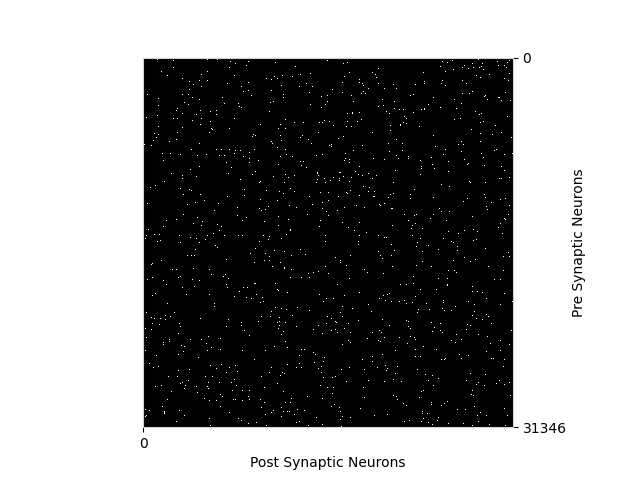
\includegraphics[width=12cm]{ER/matrix_Erdos-Renyi.png}
\caption{Sample output from the \ER model based on the statistics of the Bio-M MC}
\end{center}
\end{figure}
\subsubsection{Block Layout}
Given that each neuron pairing has an equal probability of connecting, it is unsurprising that a sample from $\mathcal{G}_{ER}$, shown in Figure 10, gives a uniform distribution of connections contained within each block. To illustrate this fact further, in Figure 11, we see each block contains approximately $0.8\%$ of the total potential connections within that block. This type of illustration where we speak purely in terms of the number of potential connections in each block is dealt with for this model only. The subsequent models in later sections will deal with Block-wise Edge Densities with respect to the proportion of connections observed in the functional graph created by the Bio-M MC. We look at this for the \ER model now.  
Now, given the distribution of edges in the blocks of the MC, it becomes clear that the block sizes are unequal. We can see this clearly from and 12(b), where we observe that each block contains a varying number of connections, ranging from around 900 to 1.2 million connections. Figure 12(a) gives the Block-wise Edge Densities. A breakdown of the TV distance of the Block-wise edge densities from the Bio-M MC can be found in section 6.4.
\begin{figure}[H]
\begin{center}
\captionsetup{justification=centering}
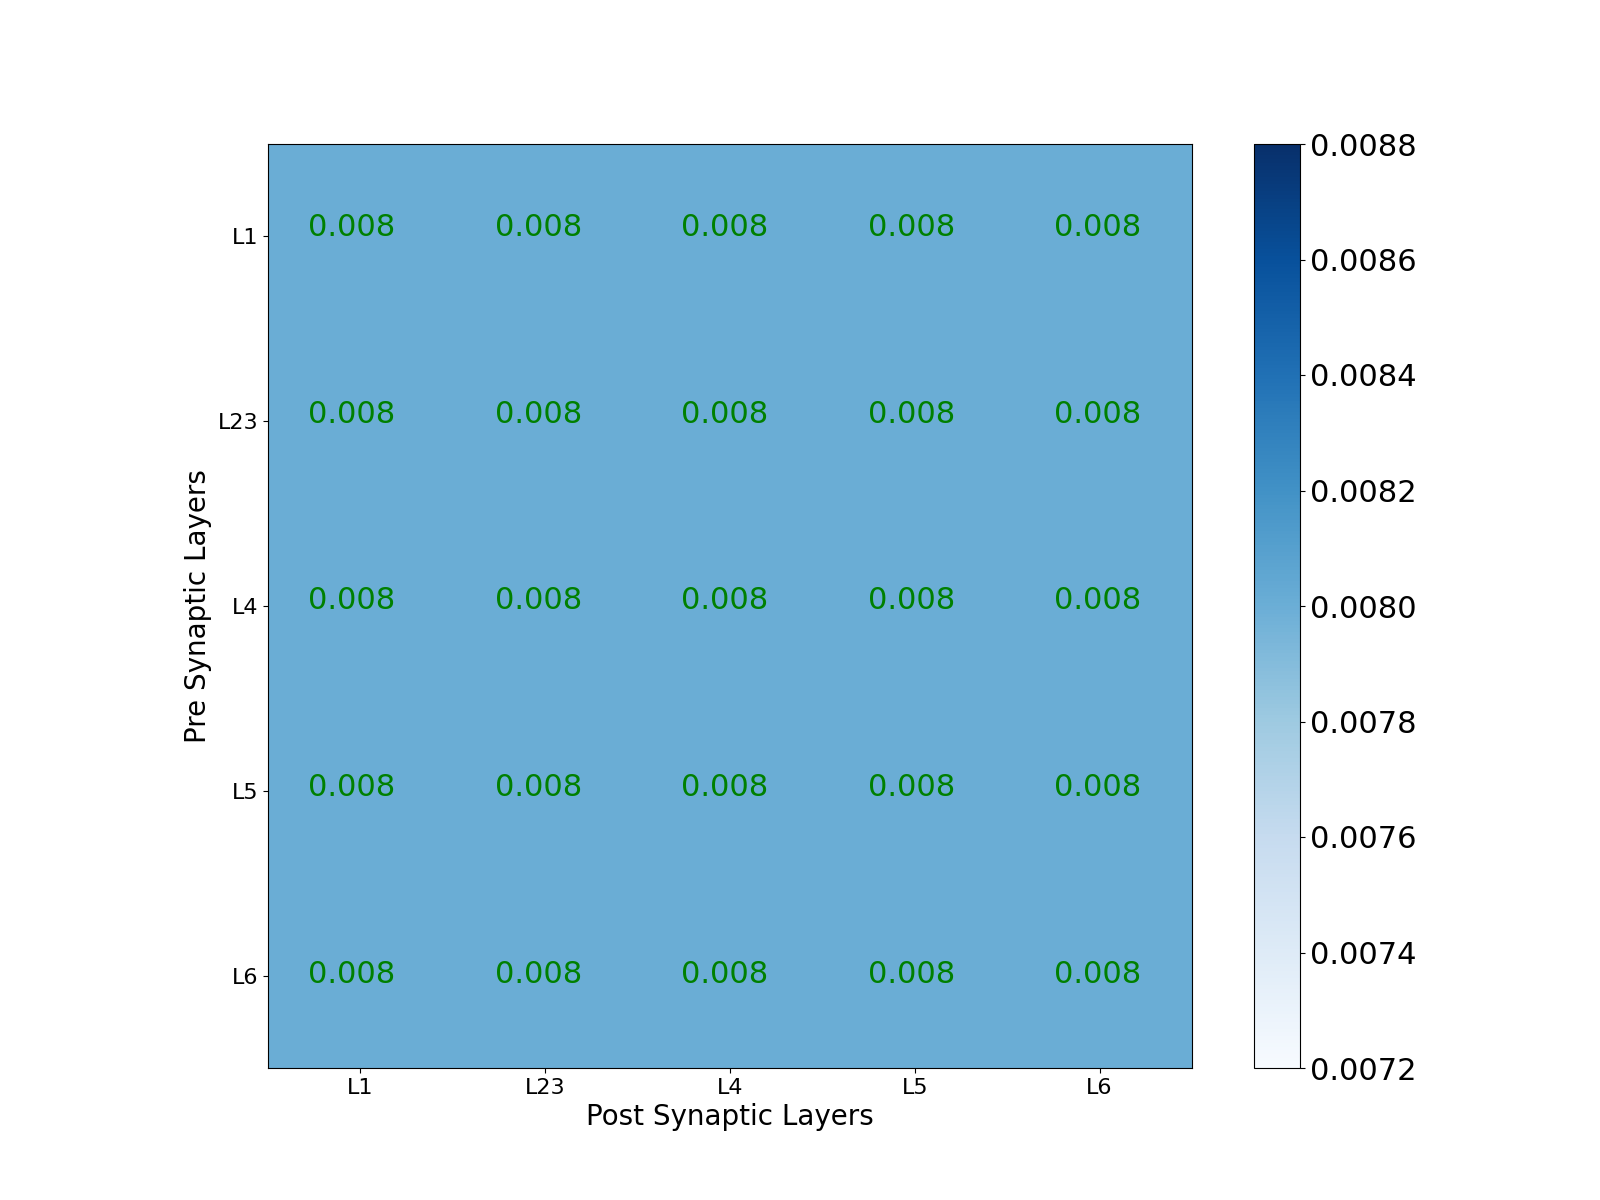
\includegraphics[width=9cm]{ER/heat_map_layer_Erdos-Renyi probability.png}
\caption{Density of edges in each block: $\frac{\text{Edges in block}}{\text{Total number of potential edges}}$}
\end{center}
\end{figure}


\begin{figure}[H]%
    \centering
    \captionsetup{justification=centering}
    \subfloat[\centering Block-wise Edge Densities ]{{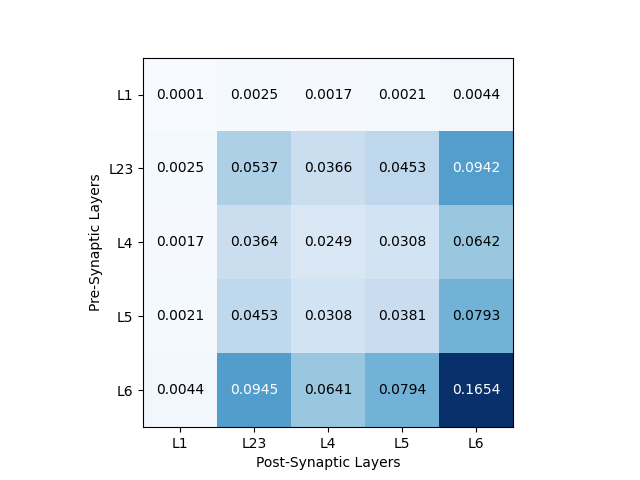
\includegraphics[width=7cm]{ER/heat_map_layer_er_test.png} }}%
    \qquad
    \subfloat[\centering Block-wise Edge Counts]{{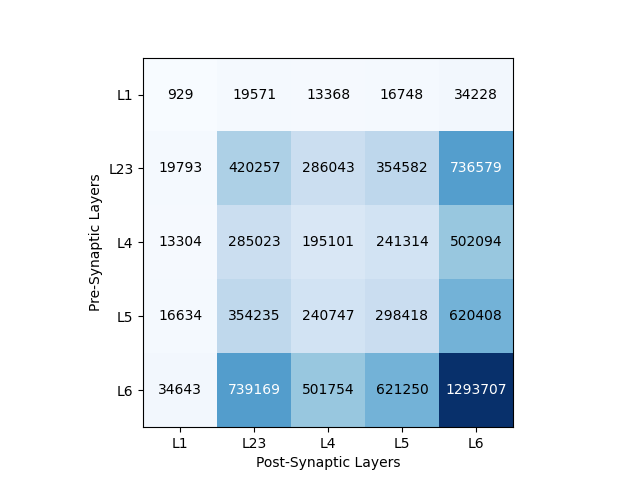
\includegraphics[width=7cm]{ER/heat_map_layer_Erdos_Renyi.png} }}%
    \caption{Connectivity by block of a random graph $\mathcal{G}_{ER}$ given by the \ER model}%
    \label{fig:example}%
\end{figure}

\subsubsection{Distance distributions}
To get an idea of the distribution of distances between neurons under the \ER model, we superimposed it onto that of the functional graph of the Bio-M MC. We computed the pairwise distances of the indexed neurons and plotted the histogram to represent these connections against what it was for the Bio-M MC in Figure 13. A metric that we use to ascertain differences here, is that of the TV distance, described in mathematical preliminaries, between the \ER model and the Bio-M MC. Here, briefly, we can state that, over 100 realisations, the mean TV distance between the \ER model and the Bio-M MC is 0.7092. This is the highest distance between a model and the MC described here. Further details about this statistic are to be found in Section 6, Results.
\begin{figure}[H]
\begin{center}
\captionsetup{justification=centering}
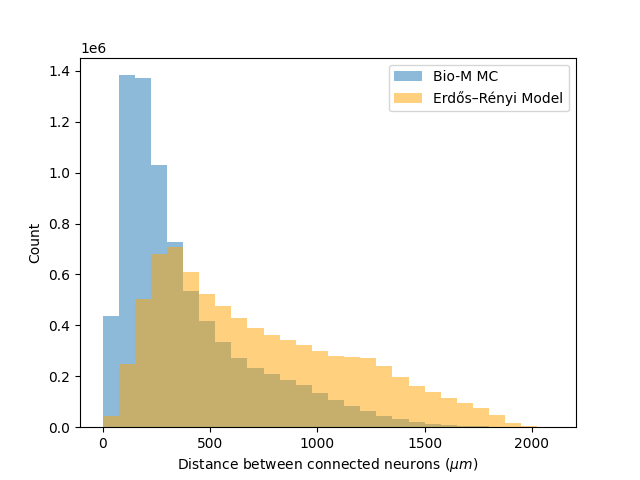
\includegraphics[width=9cm]{ER/Erdos_Renyi_dist_distr.png}
\caption{Distance distribution of connected neurons for the random graph $\mathcal{G}_{ER}$ \\if they were superimposed onto functional graph of the Bio-M MC}
\end{center}
\end{figure}

\subsubsection{Signed Degree of Neurons}
One noteworthy difference between the \ER random graph model and all the other models, as can be seen from the cumulative signed degree graphs in Figure 14, is that each neuron does not maintain the same in-degree and out-degree as that of the Bio-M MC and therefore all of our other models that preserve the in-degree and out-degree of the Bio-M MC. 

\begin{figure}[H]%
    \centering
    \captionsetup{justification=centering}
    \subfloat[\centering Realisation 1 ]{{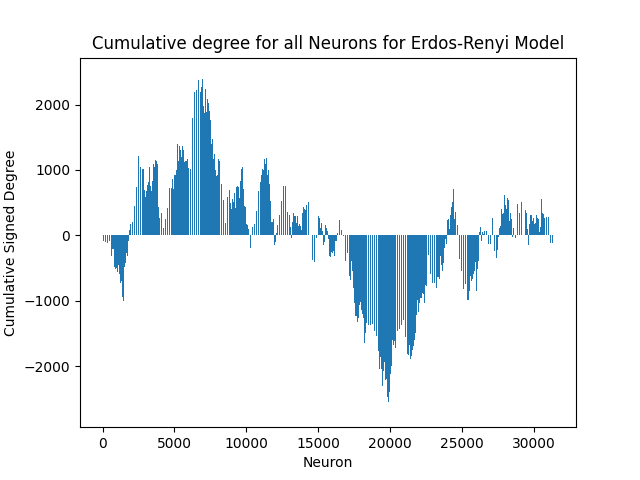
\includegraphics[width=7cm]{ER/cumsum_degree_Erdos-Renyi.png} }}%
    \qquad
    \subfloat[\centering Realisation 2]{{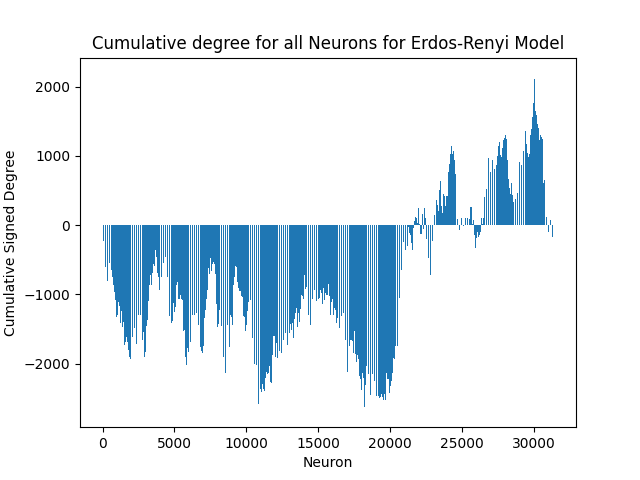
\includegraphics[width=7cm]{ER/cumsum_degree_Erdos-Renyi1.png} }}%
    \qquad
    \subfloat[\centering Realisation 3]{{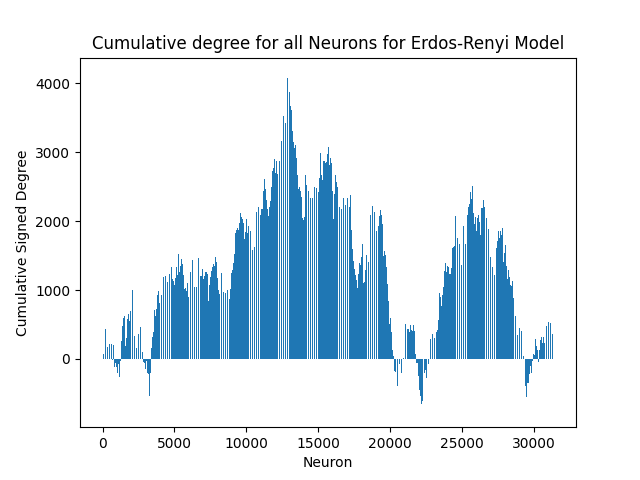
\includegraphics[width=7cm]{ER/cumsum_degree_Erdos-Renyi2.png}}}%
    \qquad
    \subfloat[\centering Realisation 4]{{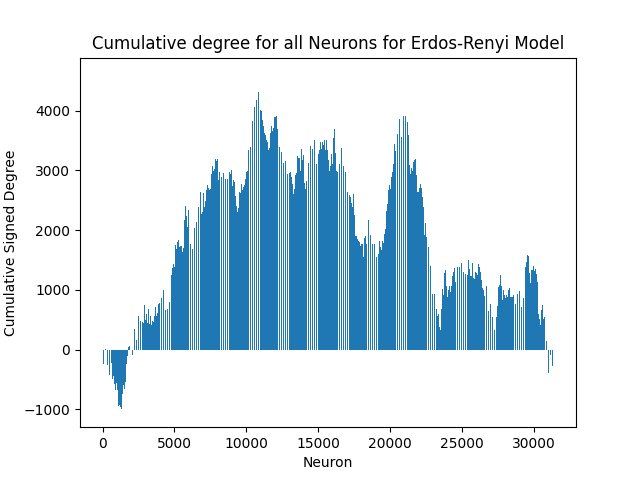
\includegraphics[width=7cm]{ER/cumsum_degree_Erdos-Renyi3.png}}}
    \caption{Realisations of the Cumulative Signed Degree for \ER random graph model}%
    \label{fig:example}%
\end{figure}










\newpage


%--------------------------------------
%--------------------------------------
%--------------------------------------
\subsection{Configuration Model}
This model reconnects the Bio-M MC using the ``cut-permute-rewire'' algorithm proposed by Watts and Strogatz \cite{WattsStrogatz1998}.

\subsubsection{Construction}
We use the ``cut-permute-rewire'' algorithm to produce samples from $\mathcal{G}_{C}$, the Configuration random graph model. This model outputs the rewired neurons by a  resampling of the connected directed edges of the Bio-M MC. By restricting ourselves to the constraints of the algorithm, this model will be able to retain the same in-degree and out-degree for each vertex as the Bio-M MC. One difference to the Bio-M MC and the General Biological model (mentioned later) however, is that we exhibit multiple connections that occur between a pair of neurons that traverse in the same direction. We allow these connections to exist so as to ensure that each neuron does indeed maintain its in-degree and out-degree. This occurs for the subsequent three models as well, namely the Geometric Configuration model, the Block Configuration model and the Block Geometric Configuration model.


\begin{figure}[H]%
    \centering
    \captionsetup{justification=centering}
    \subfloat[\centering Before configuration of small network]{{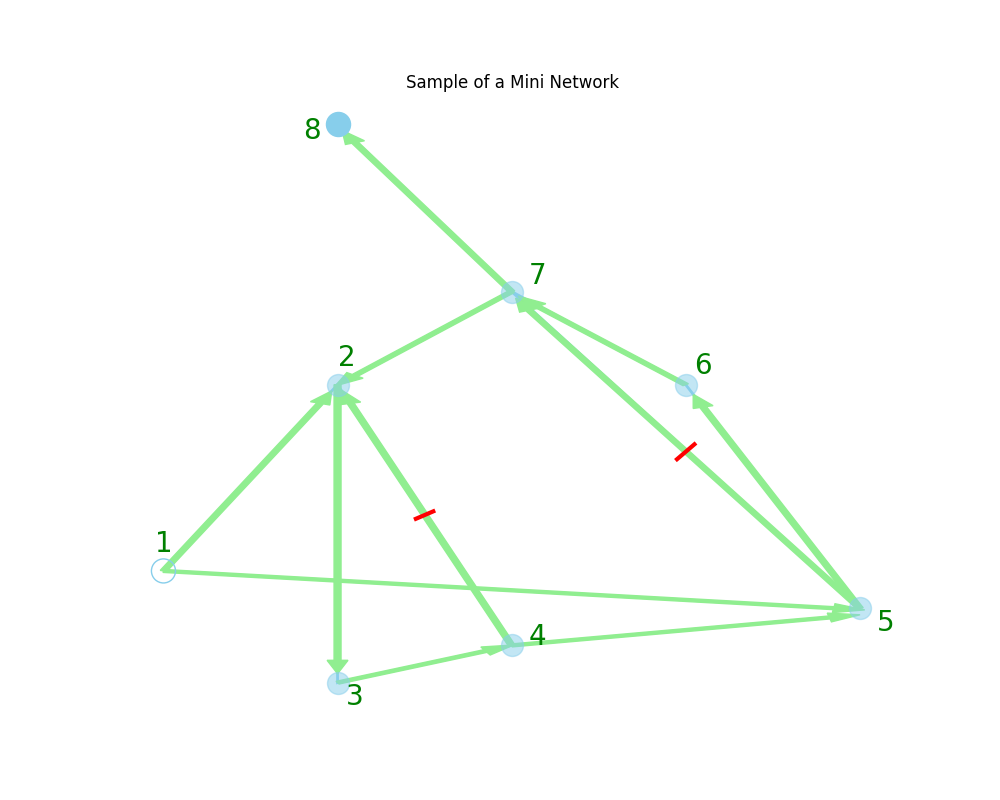
\includegraphics[width=7cm]{configuration/config_before_rewire.png} }}%
    \qquad
    \subfloat[\centering After configuration of network]{{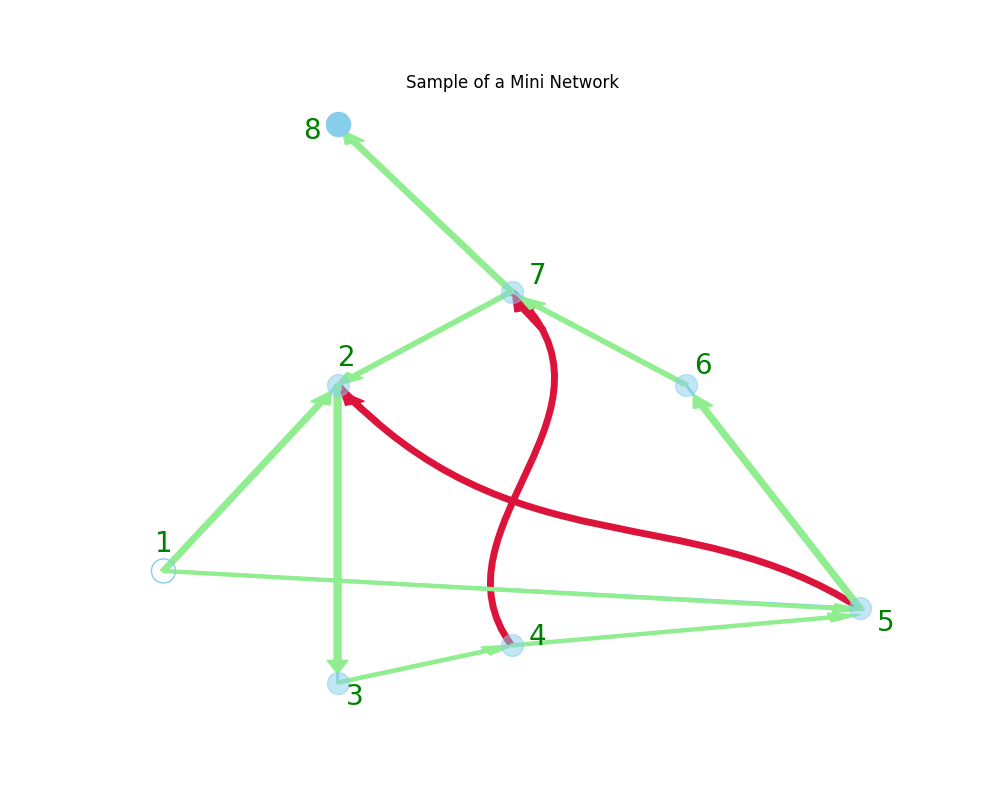
\includegraphics[width=7cm]{configuration/config_after_rewire.png} }}%
    \caption{Example of a configuration of a small version of the network}%
    \label{fig:example}%
\end{figure}

\begin{algorithm}[H]
\DontPrintSemicolon
\SetAlgoLined
\SetKwInOut{Input}{input}
\SetKwInOut{Output}{output}
\SetKwData{$E$}{$(u, v)$}
\Input{$u$, $v$}
\Output{Adjacency Matrix $M$}
\Init{}{$u \leftarrow$ Shuffle($u$)\\
$M[i,j] \leftarrow 0~\forall (i,j) \in [u][v]
$}

\ForEach{$(i,j) \in [u][v]$}
{\eIf{$i \neq j$}{$M[i,j] \leftarrow 1$}{$u \leftarrow$ Shuffle($u$)}}
\caption{$\mathcal{G_{C}}$(u, v)}
\end{algorithm}

For the ``cut-permute-rewire'' \cite{WattsStrogatz1998} algorithm to run, we first take the ordered set of edges in E, where we assign, for each $e \in E$, $\tau_1(e) = v_1$ as the pre-synaptic neurons represented by $u$ in Algorithm 2, and assign $\tau_2(e) = v_2$ as the post-synaptic neurons, represented as $v$ in Algorithm 2. We then initialise the algorithm by shuffling the order of $u$ so as to obtain a permutation of $u$, the pre-synaptic neurons. We then attempt to connect each vertex pairing providing we do not have the same vertex, that is $i \neq j$, to avoid self-loops. If we happen upon an occurrence of this, then we reshuffle the remaining vertices in $u$ and continue. Upon completion, we acquire a new ordered set of vertices contained in $u^\prime$. With this new ordered set of vertices in $u^\prime$, and the vertices in $v$, we can then form the adjacency matrix M that represents a realisation of the random graph model $\mathcal{G}_{C}$. 

\begin{figure}[H]
\begin{center}
\captionsetup{justification=centering}
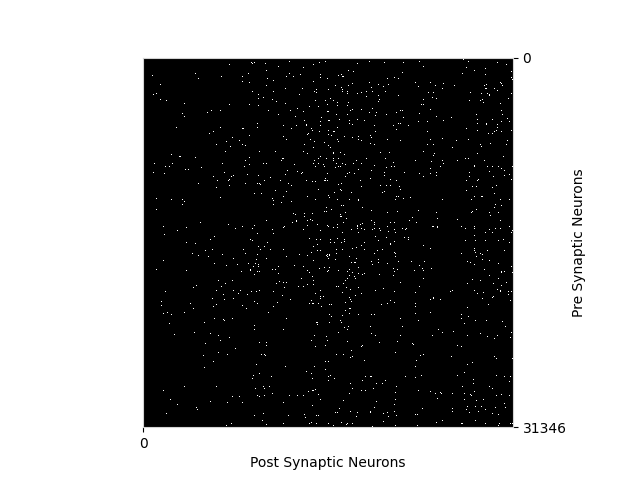
\includegraphics[width=12cm]{configuration/matrix_configuration.png}
\caption{Adjacency matrix representing a realisation of the random graph $\mathcal{G}_{C}$}
\end{center}
\end{figure}
\subsubsection{Block Layouts}
In Figure 17, we have a breakdown of the Block-wise Edge connections, both in terms of counts and in terms of density of connections within the functional graph. The density of connections concerning layer 1 amount to less than $1\%$ of all connections in a realisation of the random graph model $\mathcal{G}_{C}$ of the MC. Similarly, in relation to the structure of the Bio-M MC functional graph, the highest number of connections occur in the self-contained block of layer 6 to layer 6. Further statistics on the TV distance of the Block-wise Edge densities between the models can be found in Section 6, Results.

\begin{figure}[H]%
    \centering
    \captionsetup{justification=centering}
    \subfloat[\centering Block-wise Edge Densities]{{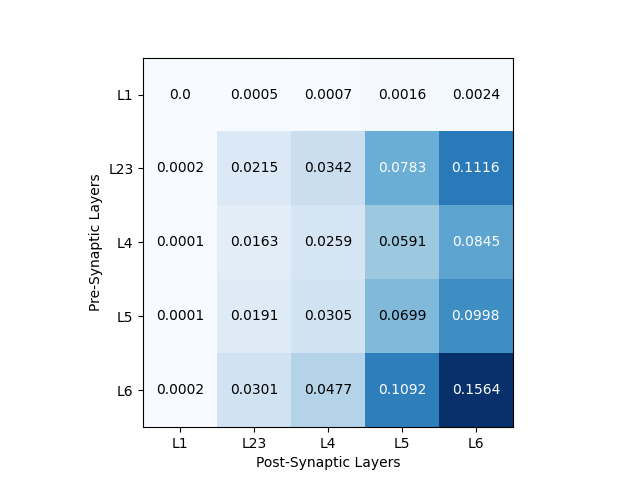
\includegraphics[width=7cm]{configuration/heat_map_layer_c_test.png} }}%
    \qquad
    \subfloat[\centering  Block-wise Edge Counts]{{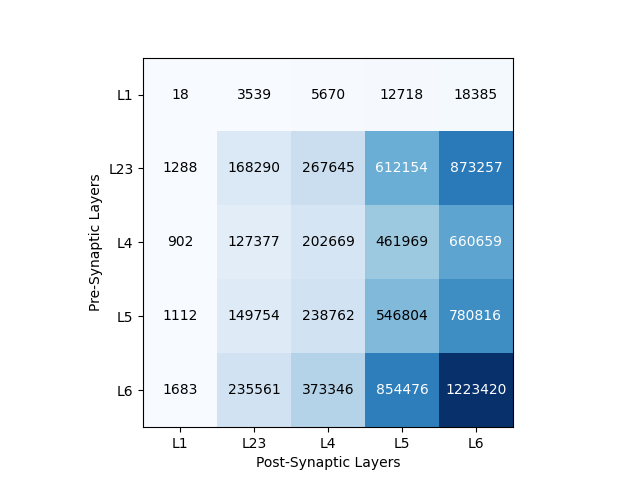
\includegraphics[width=7cm]{configuration/heat_map_layer_configuration.png} }}%
    \caption{Connectivity by block of the random graph $\mathcal{G}_{C}$ given by the Configuration Model}%
    \label{fig:example}%
\end{figure}
\subsubsection{Distance Distributions}
In Figure 18, we can also see a similar distance distribution as to that of the \ER model. As mentioned for the \ER model, we have a TV distance to the Bio-M MC. For the Configuration model, this is 0.6595. This is an improvement on the TV distance given by the \ER model. Further details are given in the Results section.
\begin{figure}[H]
\begin{center}
\captionsetup{justification=centering}
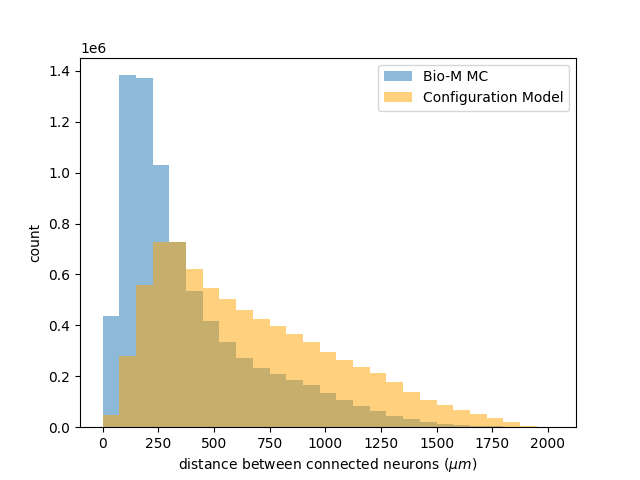
\includegraphics[width=12cm]{configuration/configuration_dist_distr.png}
\caption{Distance distribution of connected neurons for the random graph $\mathcal{G}_C$}
\end{center}
\end{figure}
\subsubsection{Signed Degree of Neurons}
From Figure 19, we see that the each neuron has maintained its in-degree and out-degree thereby following the constraints of the ``cut-permute-rewire'' \cite{WattsStrogatz1998} algorithm. 
\begin{figure}[H]%
    \centering
    \captionsetup{justification=centering}
    \subfloat[\centering Signed degree of each neuron ]{{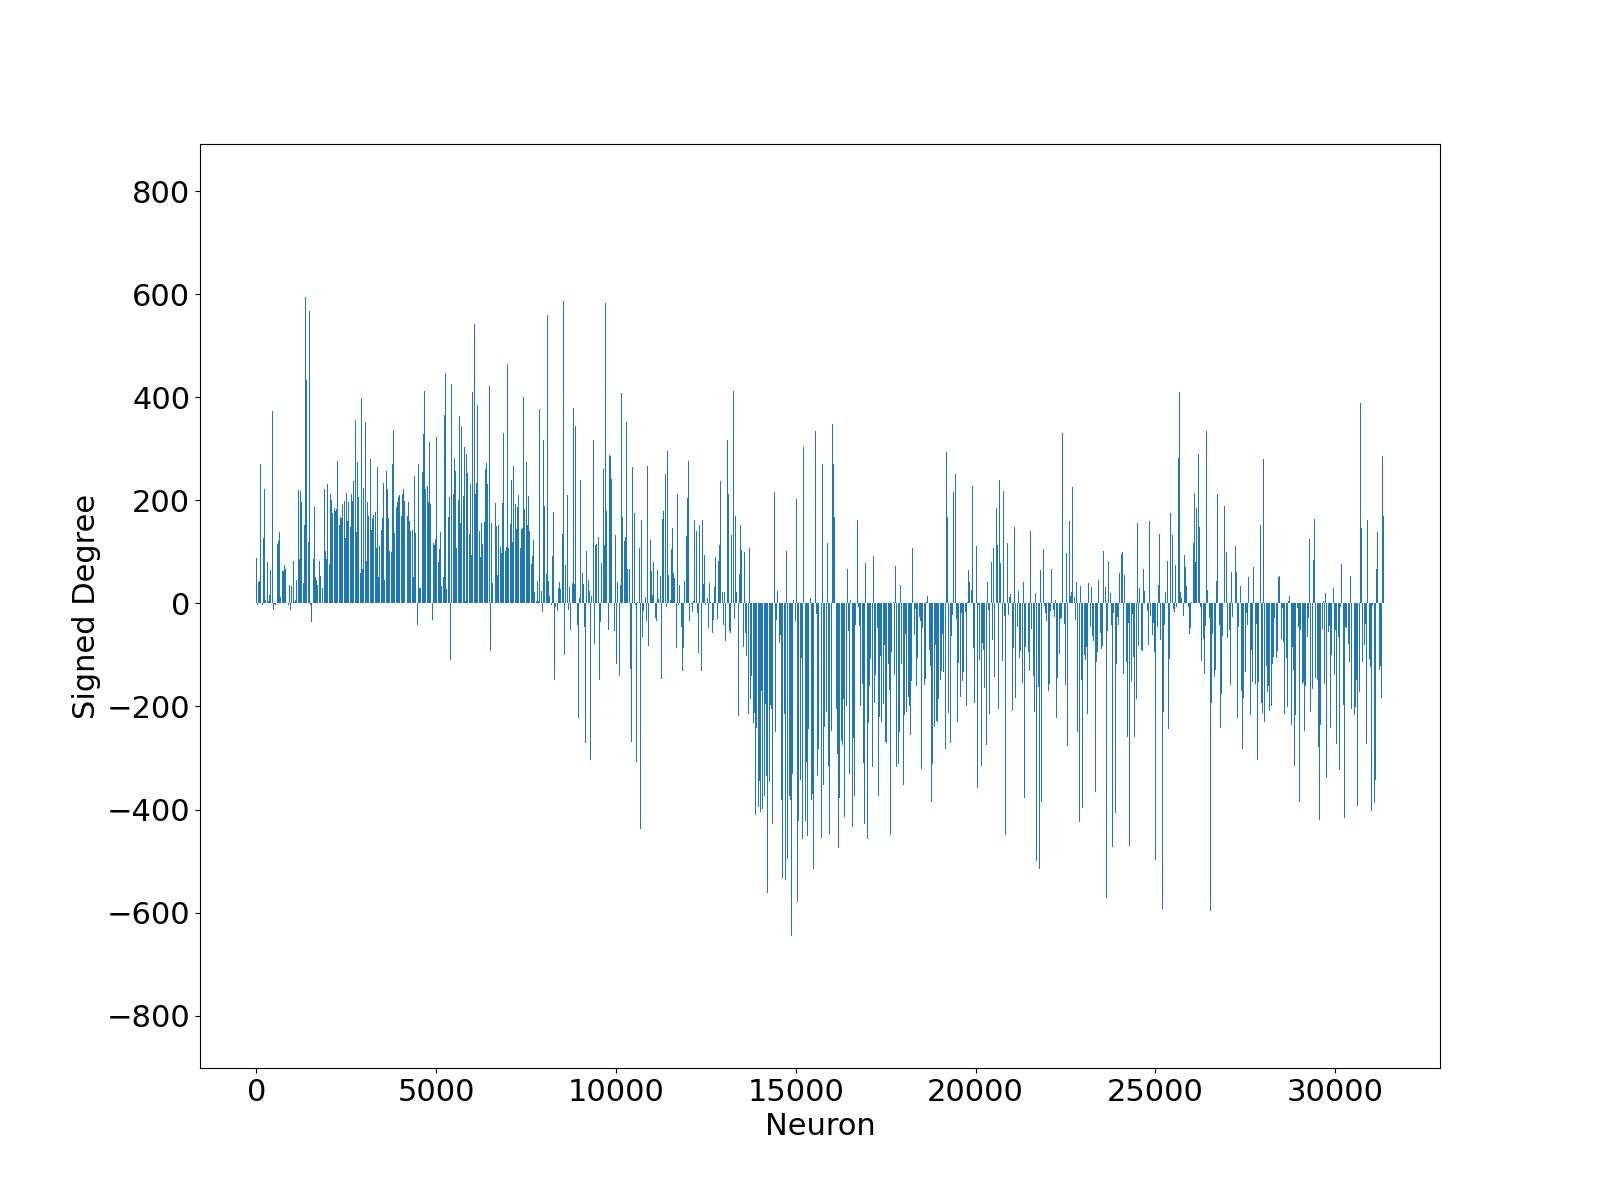
\includegraphics[width=7cm]{configuration/configuration_sd.png} }}%
    \qquad
    \subfloat[\centering Cumulative sum of the Signed Degree of the neurons in a realisation of the random graph $\mathcal{G}_{C}$]{{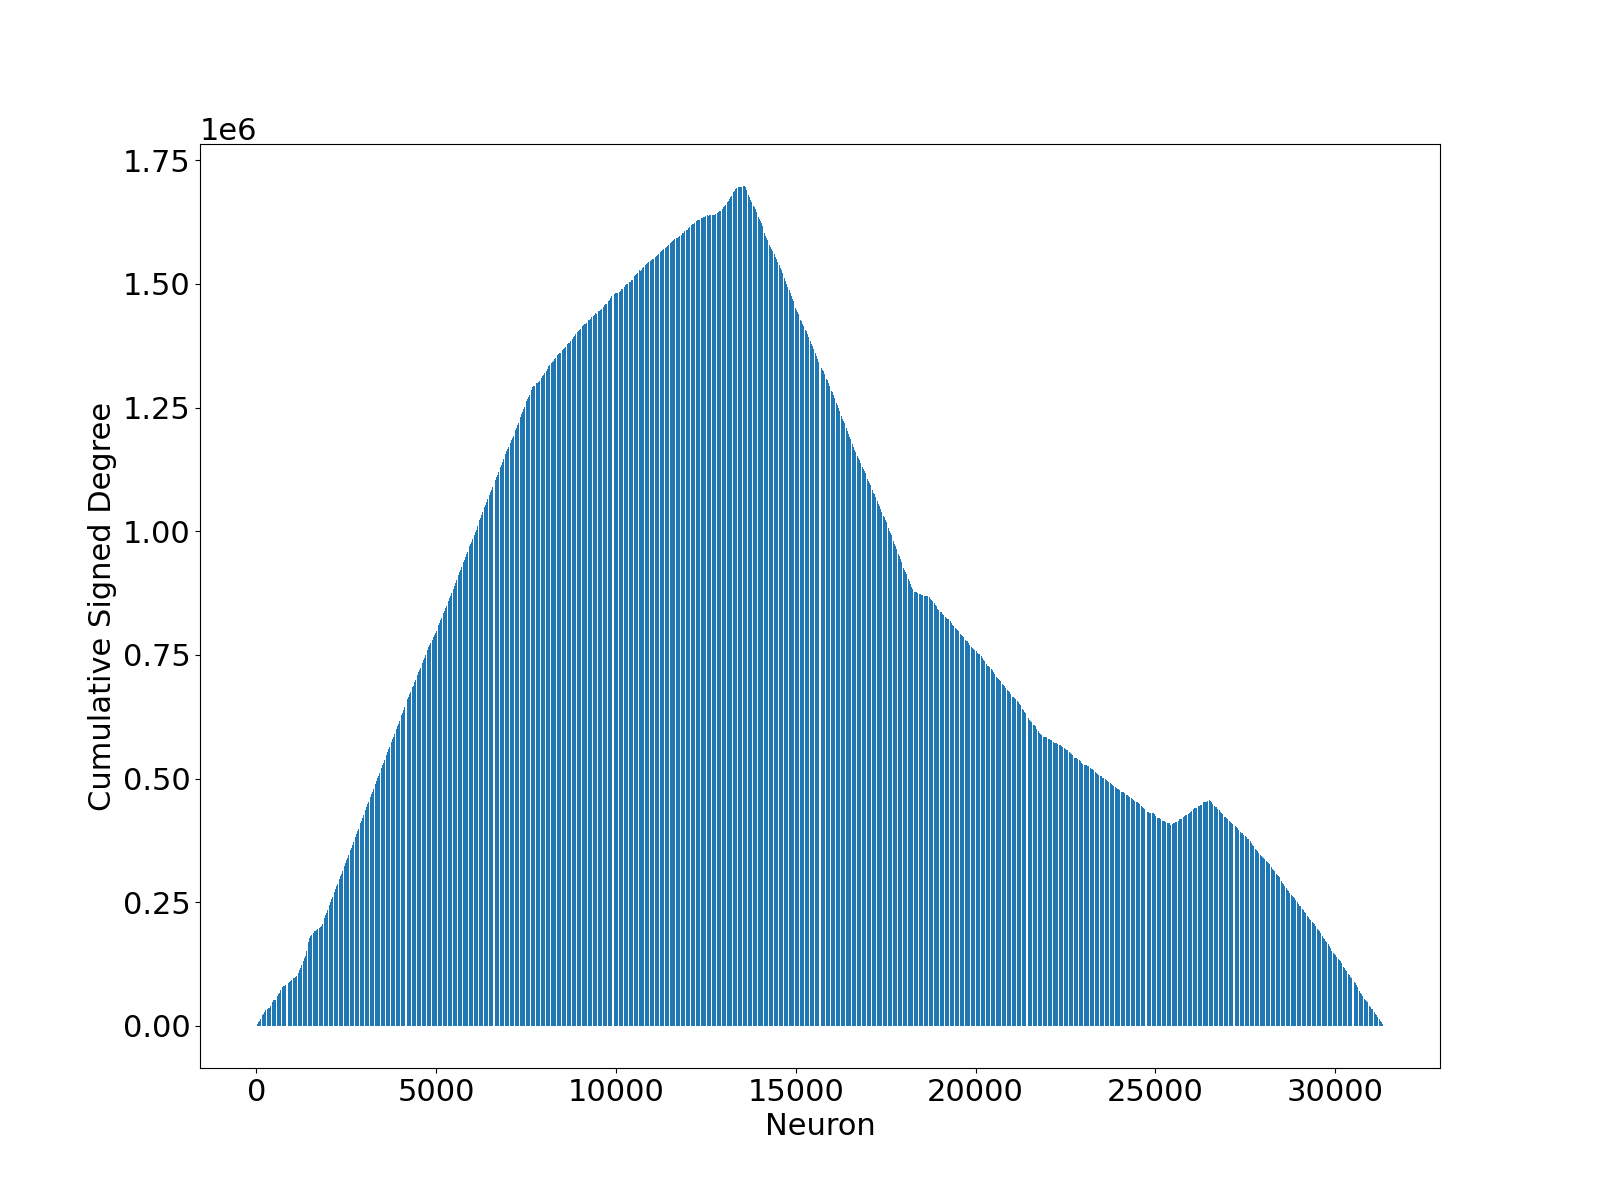
\includegraphics[width=7cm]{configuration/cumsum_degree_configuration.png} }}%
    \caption{Neuron Statistics for a realisation of the random graph $\mathcal{G}_C$}%
    \label{fig:example}%
\end{figure}



%-------------------------------------
%-------------------------------------
%-------------------------------------
\newpage
\subsection{Geometric Configuration Model}
We introduce the Geometric Configuration (GC) model here. This model uses the distances between the connected neurons in the Bio-M MC. The GC model applies the ``cut-permute-rewire'' \cite{WattsStrogatz1998} algorithm to the connected neurons in the Bio-M MC, whilst also considering a geometric constraint of their distances from one another. 
\subsubsection{Construction}
The GC model is a variation of the Configuration model. This model has the added constraint that we must also take into account the locations of the neurons, in particular their pairwise distances, involved in the Bio-M MC. In Algorithm 3, we use a probability value p, that is determined by the distance distribution given in Figure 8.

\begin{algorithm}[H]
\SetAlgoLined
\SetKwInOut{Input}{input}
\SetKwInOut{Output}{output}
\SetKwData{$E$}{$(u, v)$}
\Input{$u$, $v$, $p$, random number generator $r$}
\Output{Adjacency Matrix $M$}
\Init{}{$u \leftarrow$ Shuffle($u$)\\
$M[i,j] \leftarrow 0~\forall (i,j) \in [u][v]
$}

\ForEach{$(i, j) \in [u][v]$}
{\eIf{$i \neq j$ \textbf{and} $r < p$}
{$M[i,j] \leftarrow 1$}
{$u \leftarrow$ Shuffle($u$)}}
\caption{$\mathcal{G}_{GC}$(u, v, p) using cut-permute-rewire}
\end{algorithm}

\begin{figure}[H]
\begin{center}
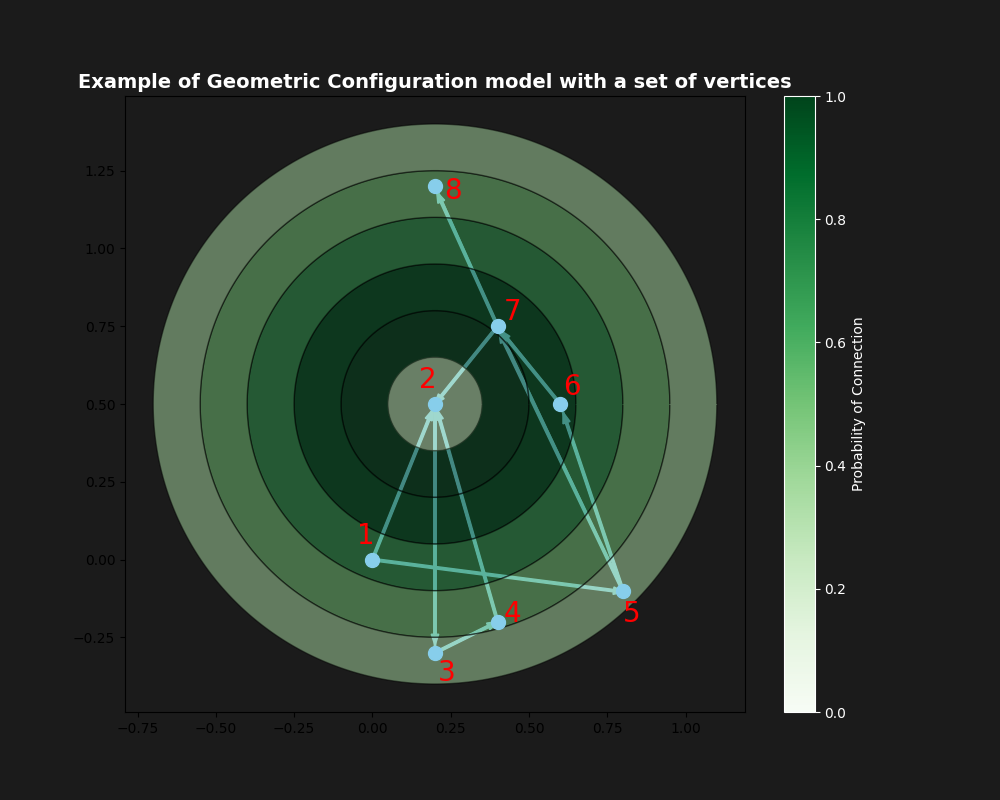
\includegraphics[width=12cm]{GC/gc_example.png}
\caption{Example of a collection of neurons and their varying probabilities of connection with neuron 2}
\end{center}
\end{figure}
As a note on the random graph model $\mathcal{G}_{GC}$, we compute the pairwise distance between each pair of vertices in E, whereby we obtain the distance distribution shown in Figure 8. This distribution shows the absolute counts of pairwise distances between neurons. This is then normalised to be used as the empirical probability distribution for connection probability between two neurons based on their pairwise distance. 
There are occasions whereby a pair of neurons may contain multiple connections heading in the same direction and that these are included in order to make sure we maintain the same in-degree and out-degree for each neuron.
\begin{figure}[H]
\begin{center}
\captionsetup{justification=centering}
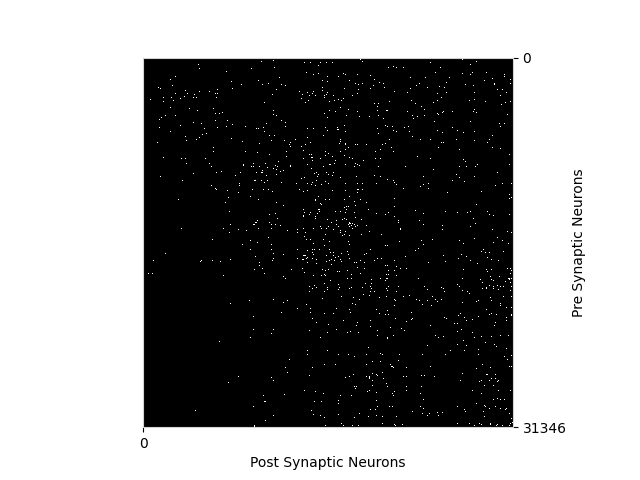
\includegraphics[width=12cm]{GC/matrix_GC.png}
\caption{Adjacency matrix M of a realisation of the random graph $\mathcal{G}_{GC}$}
\end{center}
\end{figure}
\subsubsection{Block Layouts}
Figure 22 gives the breakdown of Block-wise Edge connections, again, both in terms of counts and in terms of densities of the functional graph. Once again, we can see a small proportion of edges are contained in layer 1 and that the vast majority of edges are within layer 6. The TV distance of the Block-wise Edge densities resulted in a similar distribution of values to the Configuration Model relatively speaking. However, the vast majority of blocks here observed smaller TV distances than the Configuration Model, by a factor of 10 or more. Further details can be found in Section 6, Results.

\begin{figure}[H]%
    \centering
    \captionsetup{justification=centering}
    \subfloat[\centering Block-wise Edge Densities]{{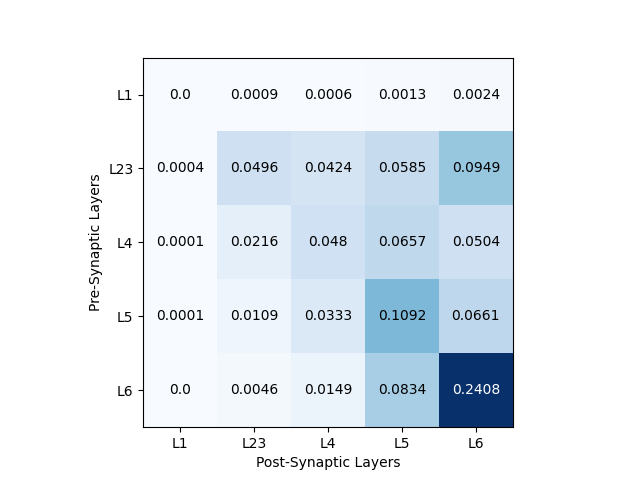
\includegraphics[width=7cm]{GC/heat_map_layer_gc_test.png} }}%
    \qquad
    \subfloat[\centering Block-wise Edge Counts]{{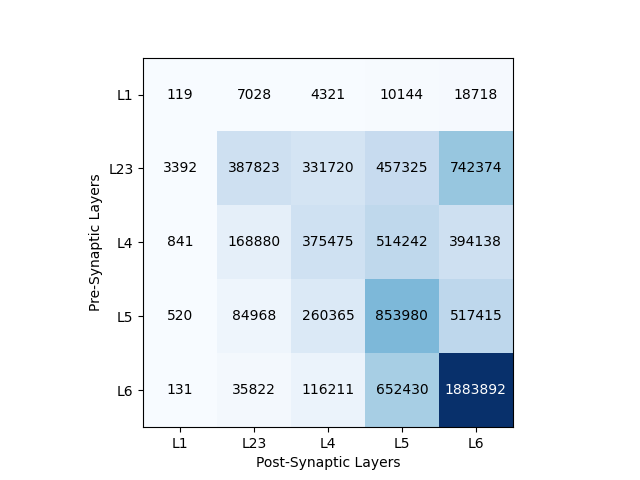
\includegraphics[width=7cm]{GC/heat_map_layer_GC.png} }}%
    \caption{Connectivity by block of the random graph $\mathcal{G}_{GC}$ given by the GC Model}%
    \label{fig:example}%
\end{figure}
\subsubsection{Distance Distribution}
We have a comparison of the distance distributions for a realisation of the Geometric Configuration model and the Bio-M MC in Figure 23. We see from this graph that the TV distance is much lower here than with the \ER model and the Configuration model, with a mean TV distance of 0.3169 after 100 realisations. This is to be expected given the construction of this model. More details of this statistic are found in section 6, Results.


\begin{figure}[H]
\begin{center}
\captionsetup{justification=centering}
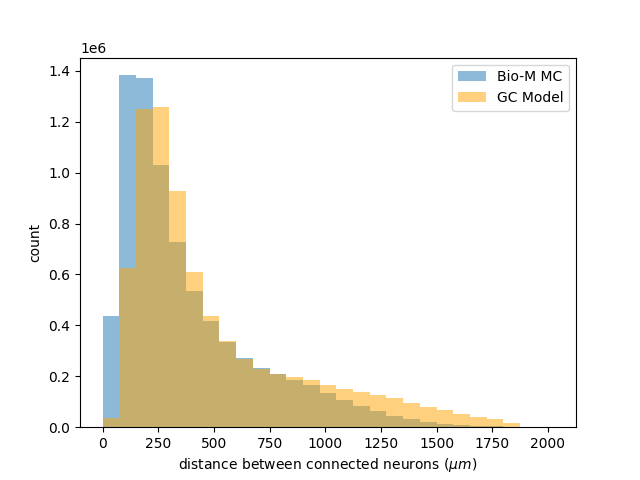
\includegraphics[width=12cm]{GC/GC_dist_distr.png}
\caption{Distance distribution of connected neurons for the random graph $\mathcal{G}_{GC}$}
\end{center}
\end{figure}

\subsubsection{Signed Degree of Neurons}
Figure 24 shows us that the in-degree and out-degree has been maintained, thereby showing that again the constraints of the  ``cut-permute-rewire'' \cite{WattsStrogatz1998} algorithm have been followed and that the graph representing the network is indeed finite.
\begin{figure}[H]%
    \centering
    \captionsetup{justification=centering}
    \subfloat[\centering Signed degree for each neuron ]{{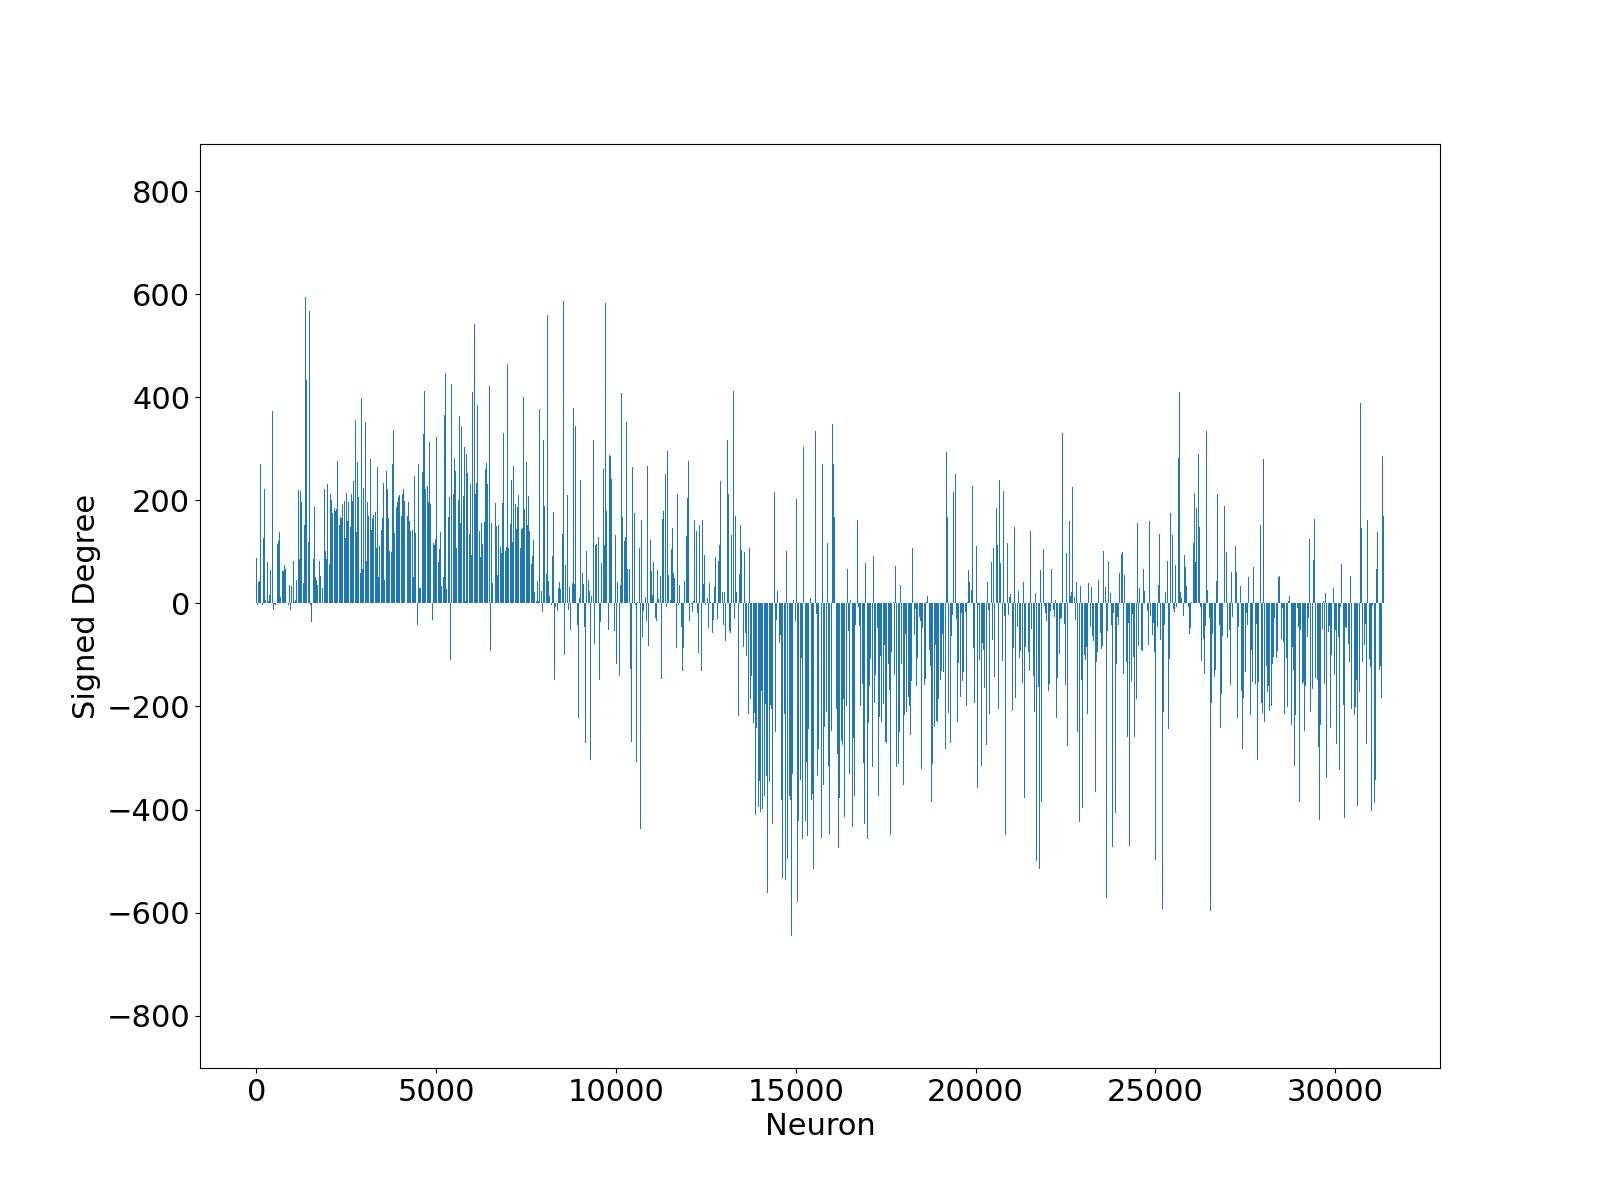
\includegraphics[width=7cm]{GC/GC_sd.png} }}%
    \qquad
    \subfloat[\centering Cumulative sum of the Signed Degree of the neurons in a realisation of the random graph $\mathcal{G}_{GC}$]{{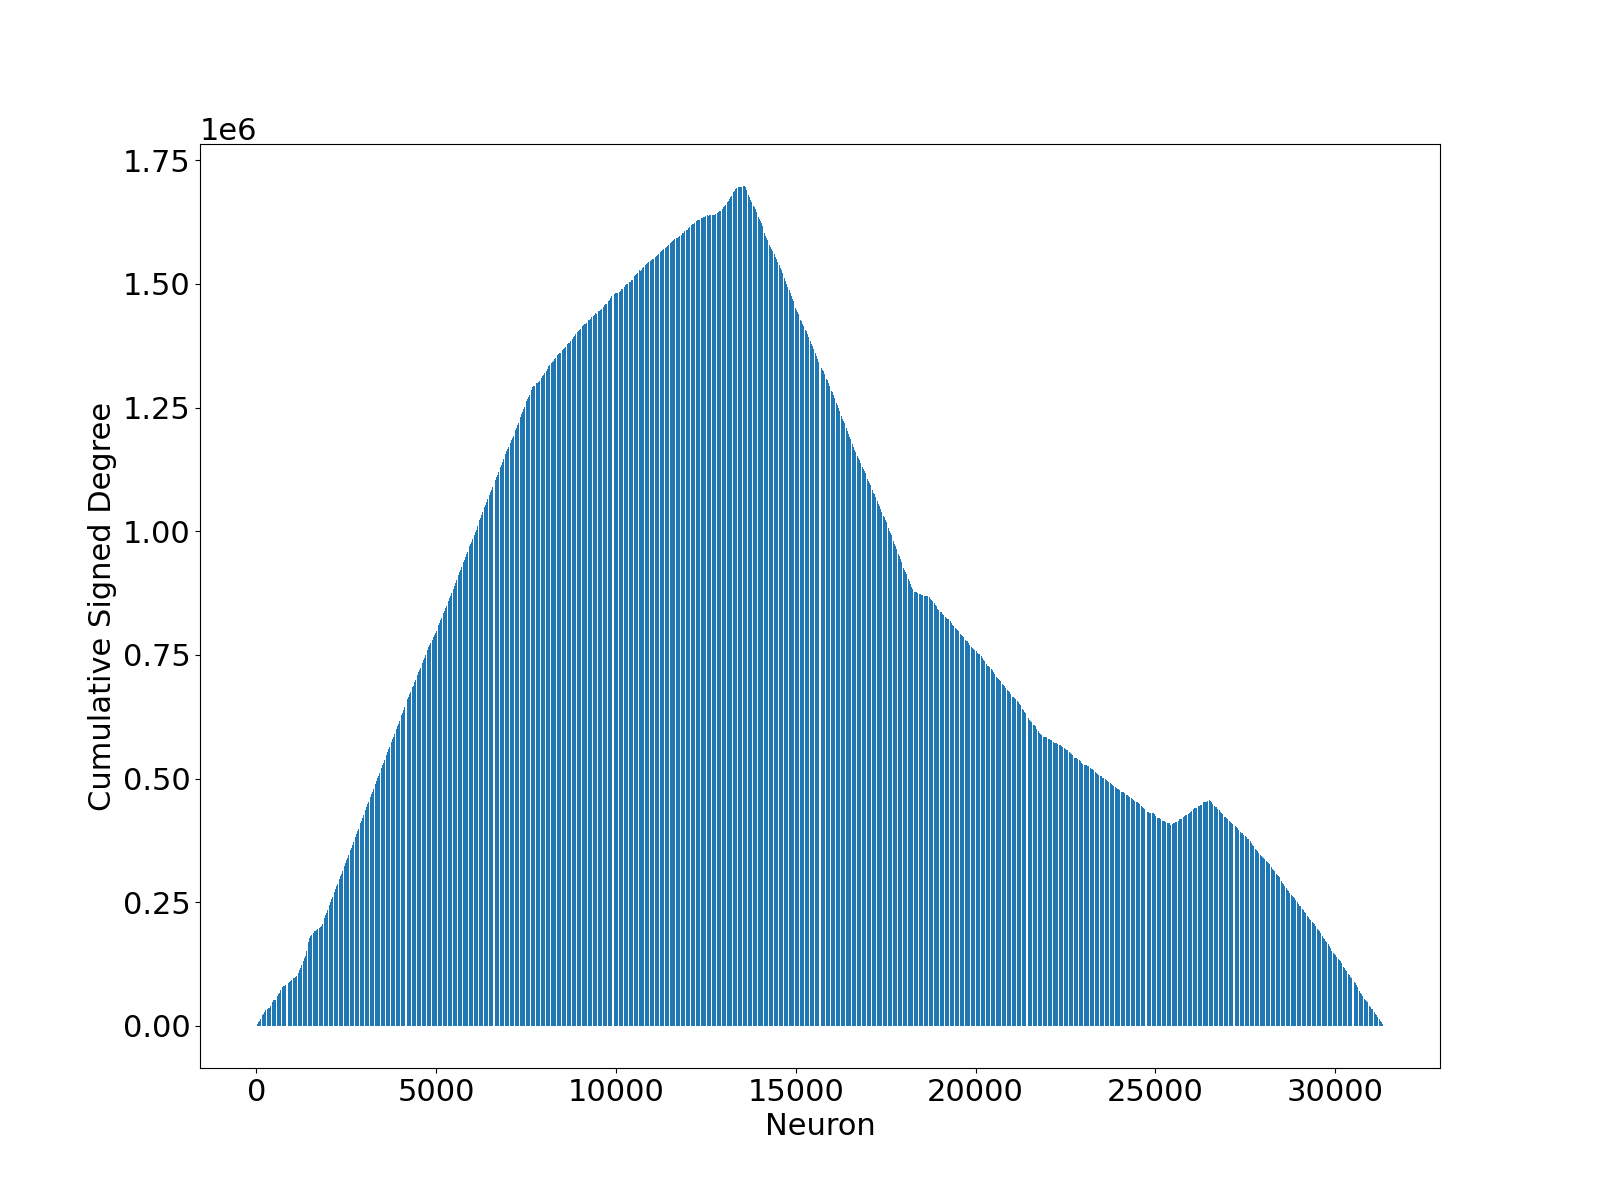
\includegraphics[width=7cm]{GC/cumsum_degree_GC.png} }}%
    \caption{Neuron statistics for the random graph $\mathcal{G}_{GC}$}%
    \label{fig:example}%
\end{figure}


 
\newpage
\subsection{Block Configuration Model}
In this section, we describe the Block Configuration model. This model uses the biological constraint of splitting up the MC into blocks comprising pre-synaptic neurons in a layer, say $i$, to post-synaptic neurons in a layer, say $j$ and using the ``cut-permute-rewire'' \cite{WattsStrogatz1998} algorithm in each block so that the layer-specific in-degrees and out-degrees for each neuron in each block is preserved, thereby seeing to it that this also remains the case for the entire random graph $\mathcal{G}_{BC}$.

\subsubsection{Construction}
The Block Configuration model is a hybrid of both the General Biological model (discussed later) and the Configuration model. This model divides up the connectome by layer rather than by morphological type, as was the case in the General Biological model and uses the ``cut-permute-rewire'' \cite{WattsStrogatz1998} algorithm. 

The construction process of the Block Configuration model begins with dividing up the MC into its 25 blocks, as shown in Figure 6. This means that we take a subset of vertices V and edges E from the Bio-M MC for each block. For each subset, we apply Algorithm 2. The resulting ordered sets $u^\prime$ and $v$ are then stored until the algorithm has been applied to all 25 blocks. On completion, these 25 blocks containing the ordered sets of vertices, are then used to construct a realisation of the random graph $\mathcal{G_{BC}}$.


\begin{figure}[H]
\begin{center}
\captionsetup{justification=centering}
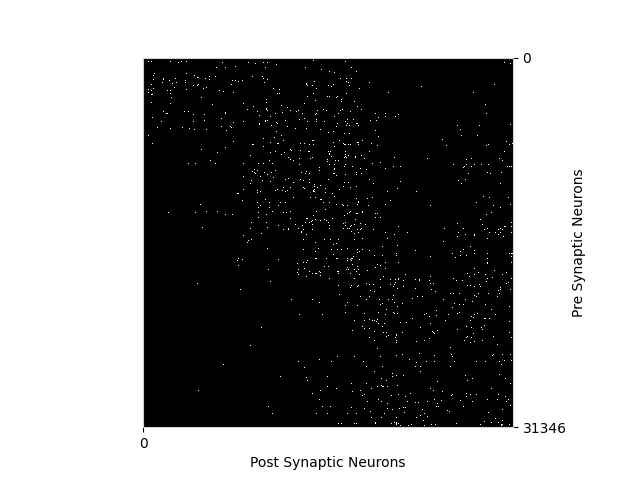
\includegraphics[width=12cm]{BC/matrix_Block_Configuration.png}
\caption{Adjacency Matrix M representing a realisation of the random graph $\mathcal{G}_{BC}$}
\end{center}
\end{figure}

\subsubsection{Block Layouts}
Given that we have subdivided the MC into 25 blocks on a layer by layer basis, the number of edges contained in each block will be precisely the same as the Bio-M MC. This is shown in Section 6, where we detail the TV distance for Block-wise Edge densities between this model and the Bio-M MC. Likewise with the Configuration Model and the Geometric Configuration Model previously, we observe pairwise neurons with multiple connections in the same direction.
\begin{figure}[H]%
    \centering
    \captionsetup{justification=centering}
    \subfloat[\centering Block-wise Edge Densities]{{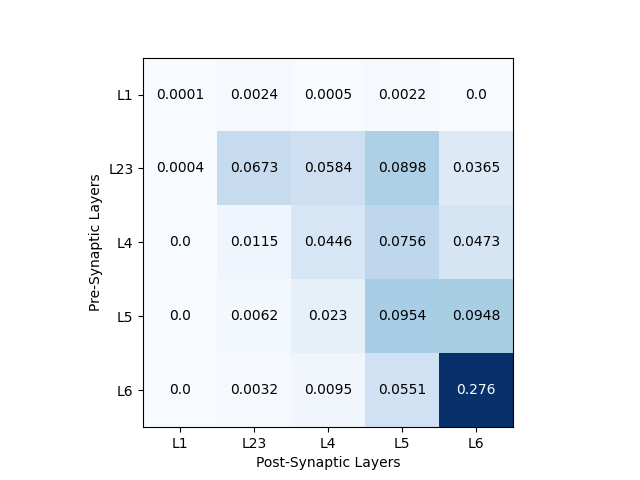
\includegraphics[width=7cm]{BC/heat_map_layer_bc_test.png} }}%
    \qquad
    \subfloat[\centering Block-wise Edge Counts ]{{\includegraphics[width=7cm]{BC/heat_map_layer_Block.png} }}%
    \caption{Connectivity by block of the random graph $\mathcal{G}_{BC}$ given by the BC model}%
    \label{fig:example}%
\end{figure}
\subsubsection{Distance Distribution}
After 100 realisations of the Block Configuration model were observed, this yielded a mean TV distance of 0.3937. This is a large improvement on the \ER model and the Configuration model, however, weaker than the GC Model. Despite not allowing for a geometrical constraint here in terms of how a pair of neurons connect, it is clear that by dividing up the MC into these blocks plays a similar role in geometrically constraining the connections since we are only able to rearrange the connections in these specific blocks. 
\begin{figure}[H]
\begin{center}
\captionsetup{justification=centering}
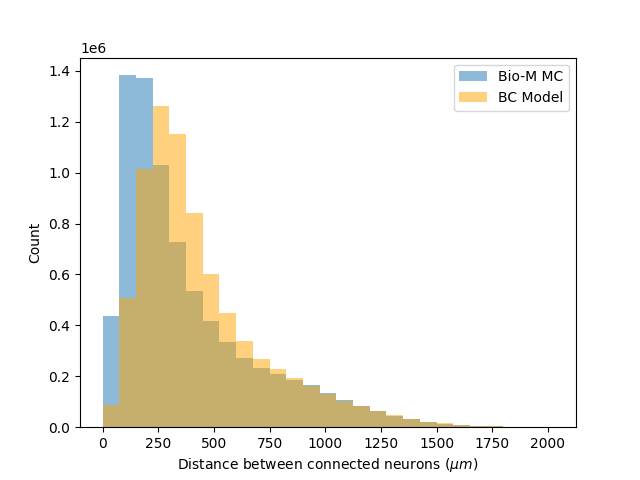
\includegraphics[width=12cm]{BC/Block_dist_distr.png}
\caption{Distance distribution of connected neurons for the random graph $\mathcal{G}_{BC}$}
\end{center}
\end{figure}

\subsubsection{Signed Degree of Neurons}
As mentioned at the head of this subsection, we have the same in-degrees and out-degrees for each neuron in each block and thereby ensuring the case for the whole random graph. \begin{figure}[H]%
    \centering
    \captionsetup{justification=centering}
    \subfloat[\centering  Signed Degree of each Neuron]{{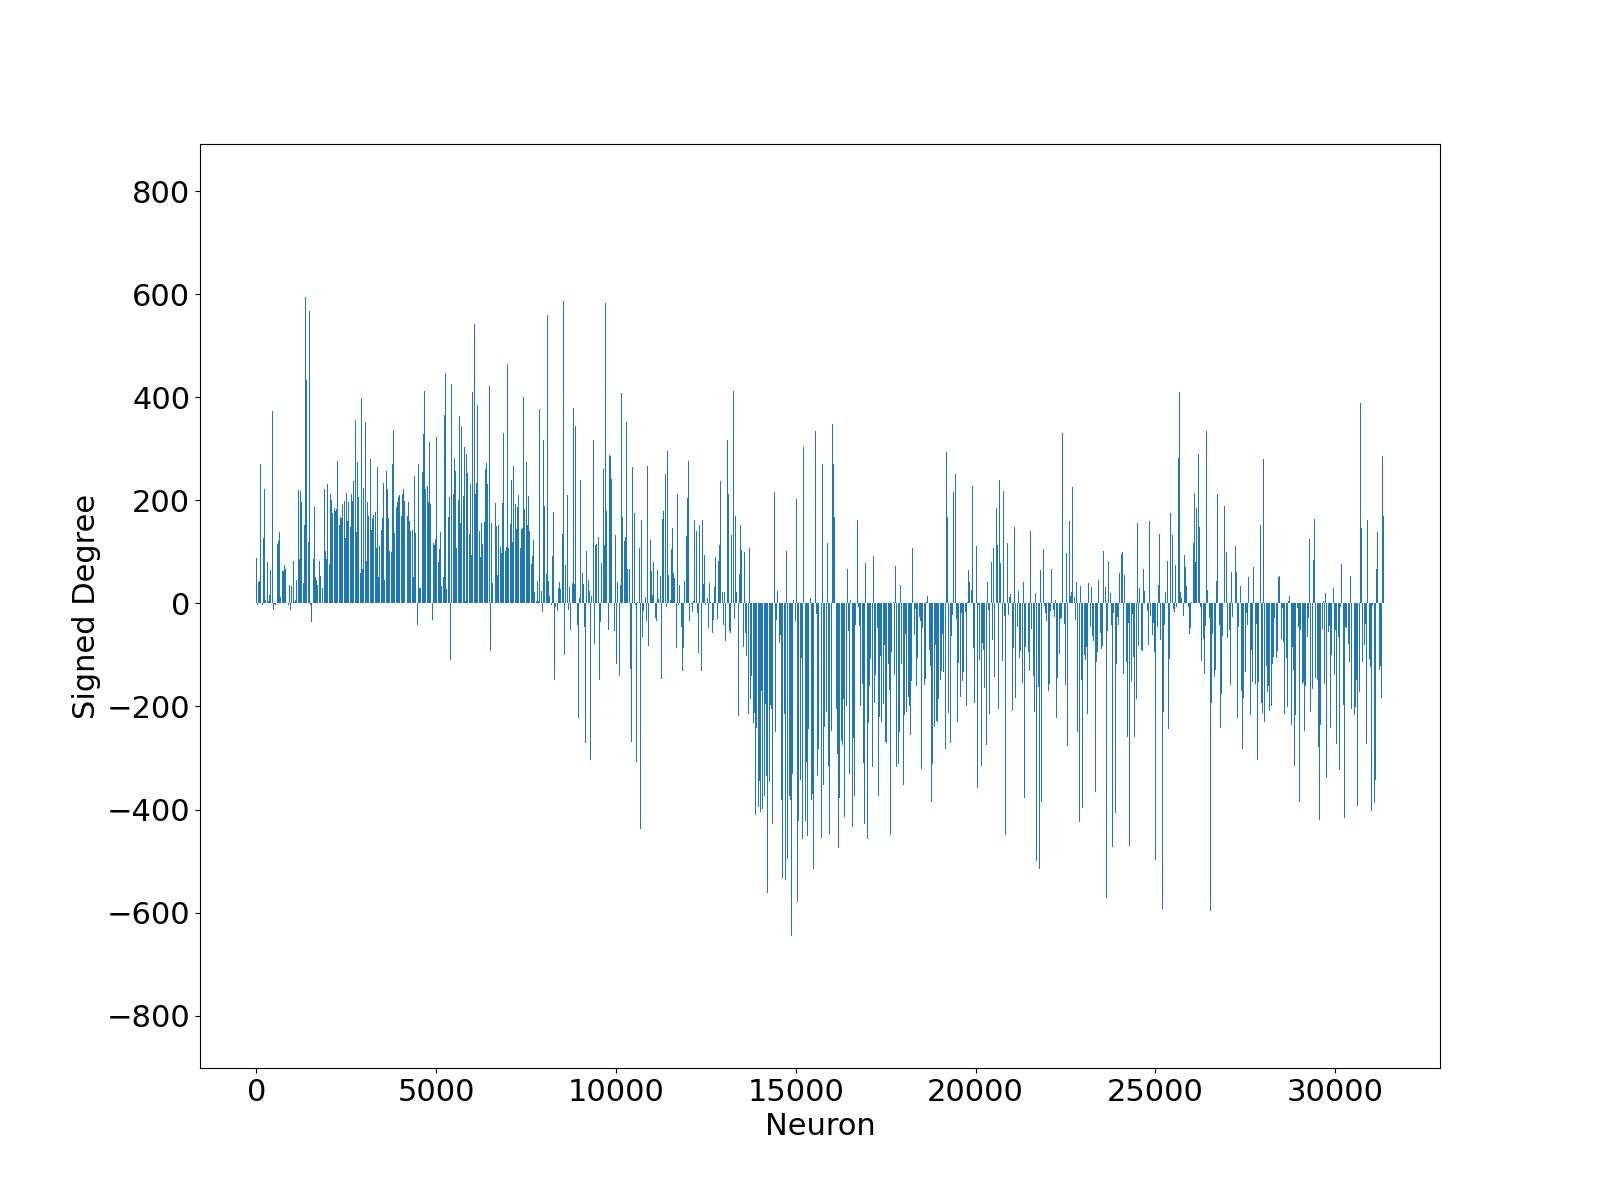
\includegraphics[width=7cm]{BC/Block_Configuration_sd.png} }}%
    \qquad
    \subfloat[\centering Cumulative sum of the Signed Degree of the neurons in a realisation of the random graph $\mathcal{G}_{BC}$ ]{{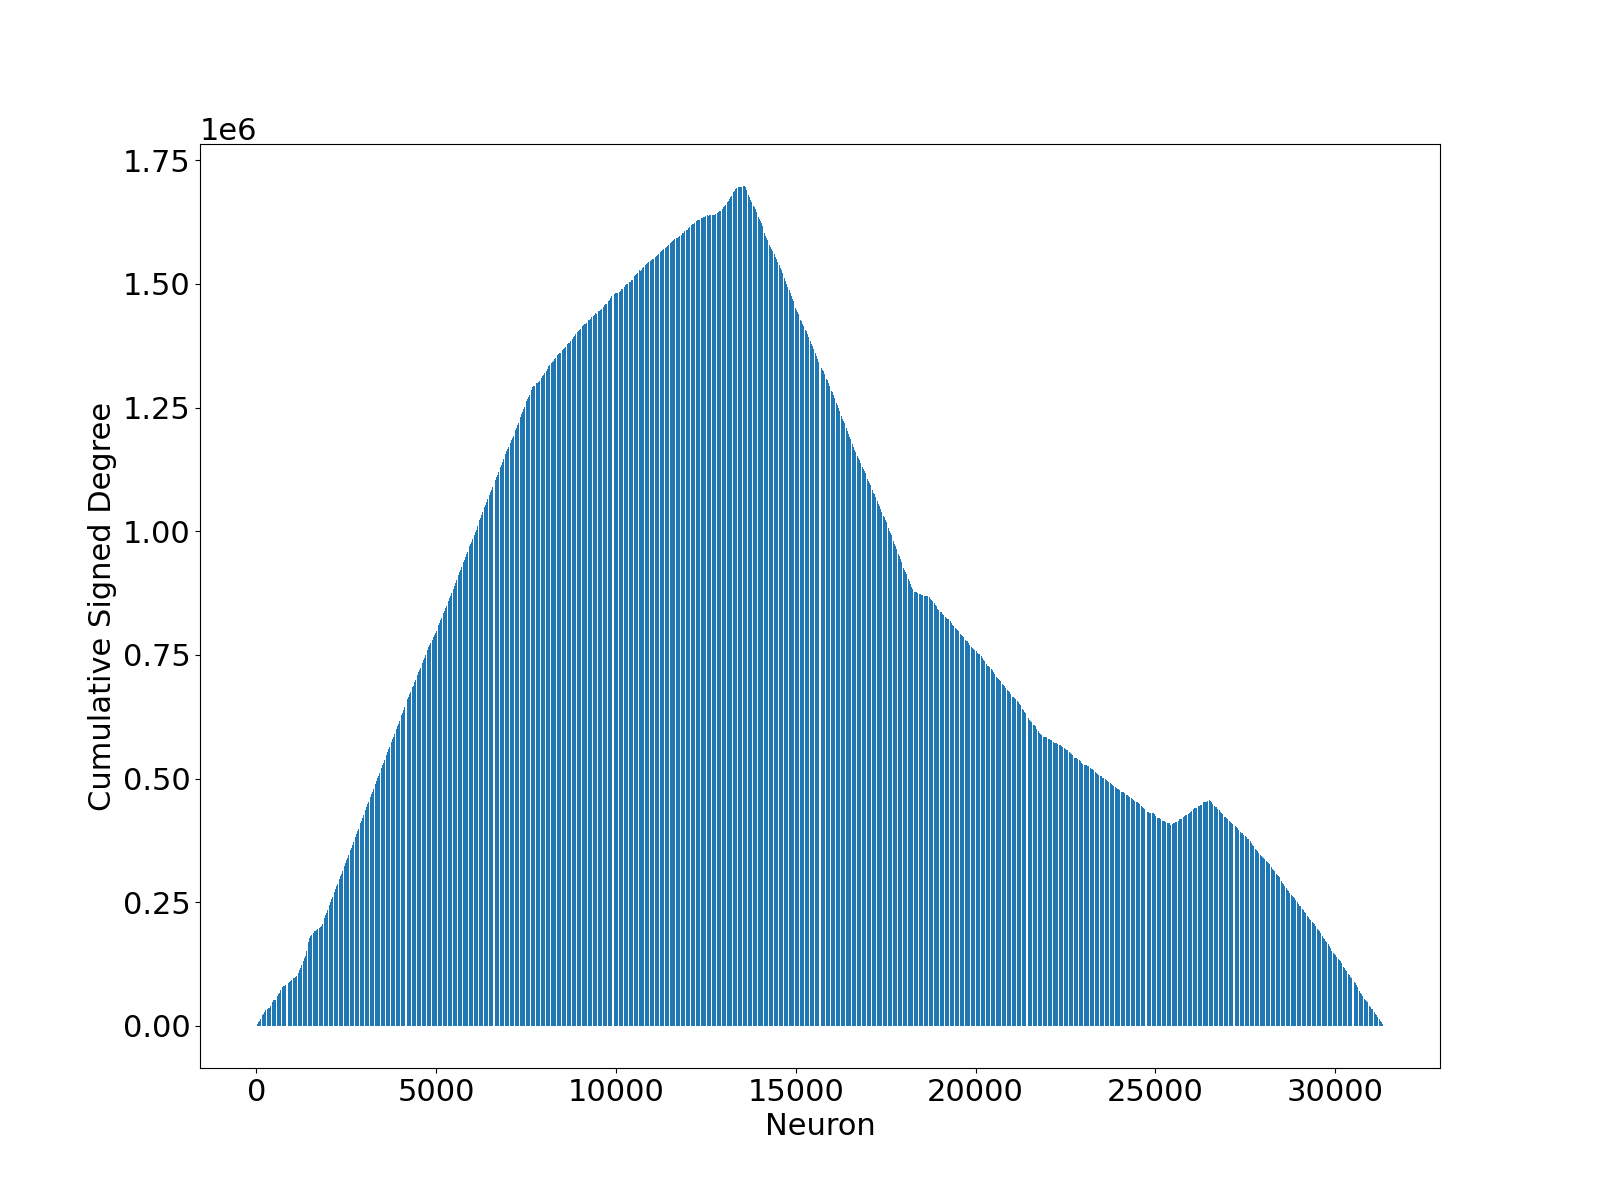
\includegraphics[width=7cm]{BC/cumsum_degree_Block_Configuration.png} }}%
    \caption{Neuron statistics for the random graph $\mathcal{G}_{BC}$}%
    \label{fig:example}%
\end{figure}

\newpage

\subsection{Block Geometric Configuration Model}
The Block Geometric Configuration model uses both the ``cut-permute-rewire'' \cite{WattsStrogatz1998} algorithm as well as the geometric constraint as mentioned in the GC model with a slight variation to it here. 
\subsubsection{Construction}
The final model that we have is the Block Geometric Configuration model. The first part of the construction process, is to divide the MC into blocks, as was the case for the Block Configuration model. The second part of the process, is to then compute the pairwise distances of connected neurons in each block. That is, we take the subset of vertices and edges in each block, and compute the distances between these neurons. We then apply Algorithm 2 to each block and return the corresponding subsets $u^\prime$ and $v$. Upon completion of all 25 blocks, we can then use these ordered sets of vertices to construct a realisation of the random graph model $\mathcal{G_{BGC}}$. Thus, $\mathcal{G_{BGC}}$ not only preserves the in-degrees and out-degrees layer-specifically for each neuron but also the probability of connecting neurons based on the empirical pairwise distances of connected neurons.

\begin{figure}[H]
\begin{center}
\captionsetup{justification=centering}
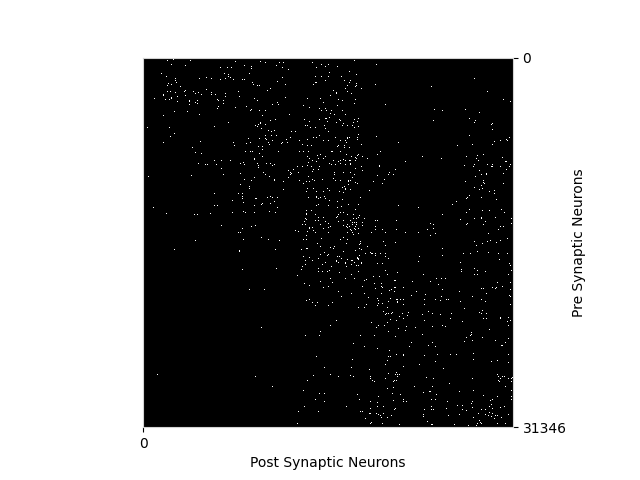
\includegraphics[width=12cm]{GBC/matrix_BGC.png}
\caption{Adjacency Matrix M representing a realisation of the random graph $\mathcal{G}_{BGC}$}
\end{center}
\end{figure}


\subsubsection{Block Layouts}
Just as we saw for the Block Configuration model, each Block-wise Edge density gives a TV distance of 0 to the Bio-M MC. As you will see from Figure 30, the values match that of the Bio-M MC. This, like the Block Configuration model has been achieved since all edge shuffling has occurred within these blocks that we are splitting the MC up into.

\begin{figure}[H]%
    \centering
    \captionsetup{justification=centering}
    \subfloat[\centering Proportion of connections in each block ]{{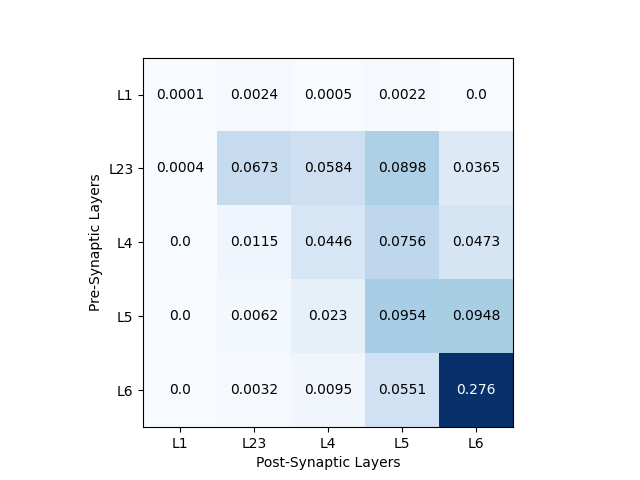
\includegraphics[width=7cm]{GBC/heat_map_layer_bgc_test.png} }}%
    \qquad
    \subfloat[\centering Total number of connections in each block ]{{\includegraphics[width=7cm]{GBC/heat_map_layer_Block.png} }}%
    \caption{Connectivity by block of the random graph $\mathcal{G}_{BGC}$ given by the BGC model}%
    \label{fig:example}%
\end{figure}

\subsubsection{Distance Distribution}

Figure 31 reveals a very similar distribution for the BGC model in comparison to the BC model. This, perhaps suggests that the geometric constraint has already been taken care of by splitting up the MC into these layer by layer blocks. Over 100 realisations of the BGC model yielded a mean TV distance of 0.3937. This is only marginally better than the BC model. Details of these differences are contained in Section 6, Results.

\begin{figure}[H]
\begin{center}
\captionsetup{justification=centering}
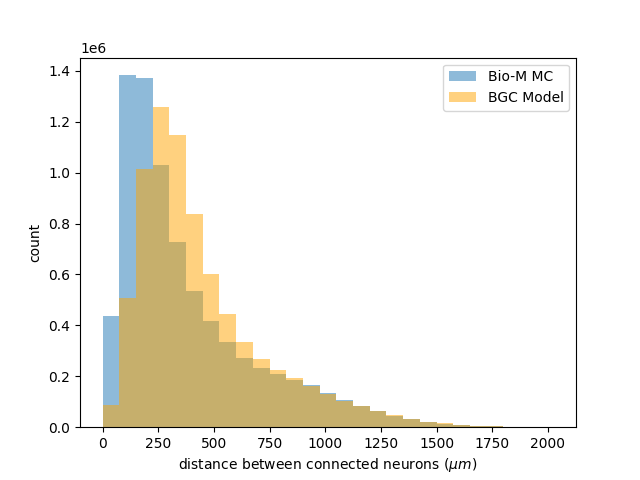
\includegraphics[width=12cm]{GBC/Block_dist_distr.png}
\caption{Distance distribution of connected neurons for the random graph $\mathcal{G}_{BGC}$}
\end{center}
\end{figure}

\subsubsection{Signed Degree of Neurons}
Just as with all the other models, we have the same in-degree and out-degree for each neuron as described by the plots in Figure 32. 

\begin{figure}[H]%
    \centering
    \captionsetup{justification=centering}
    \subfloat[\centering Signed Degree of each Neuron]{{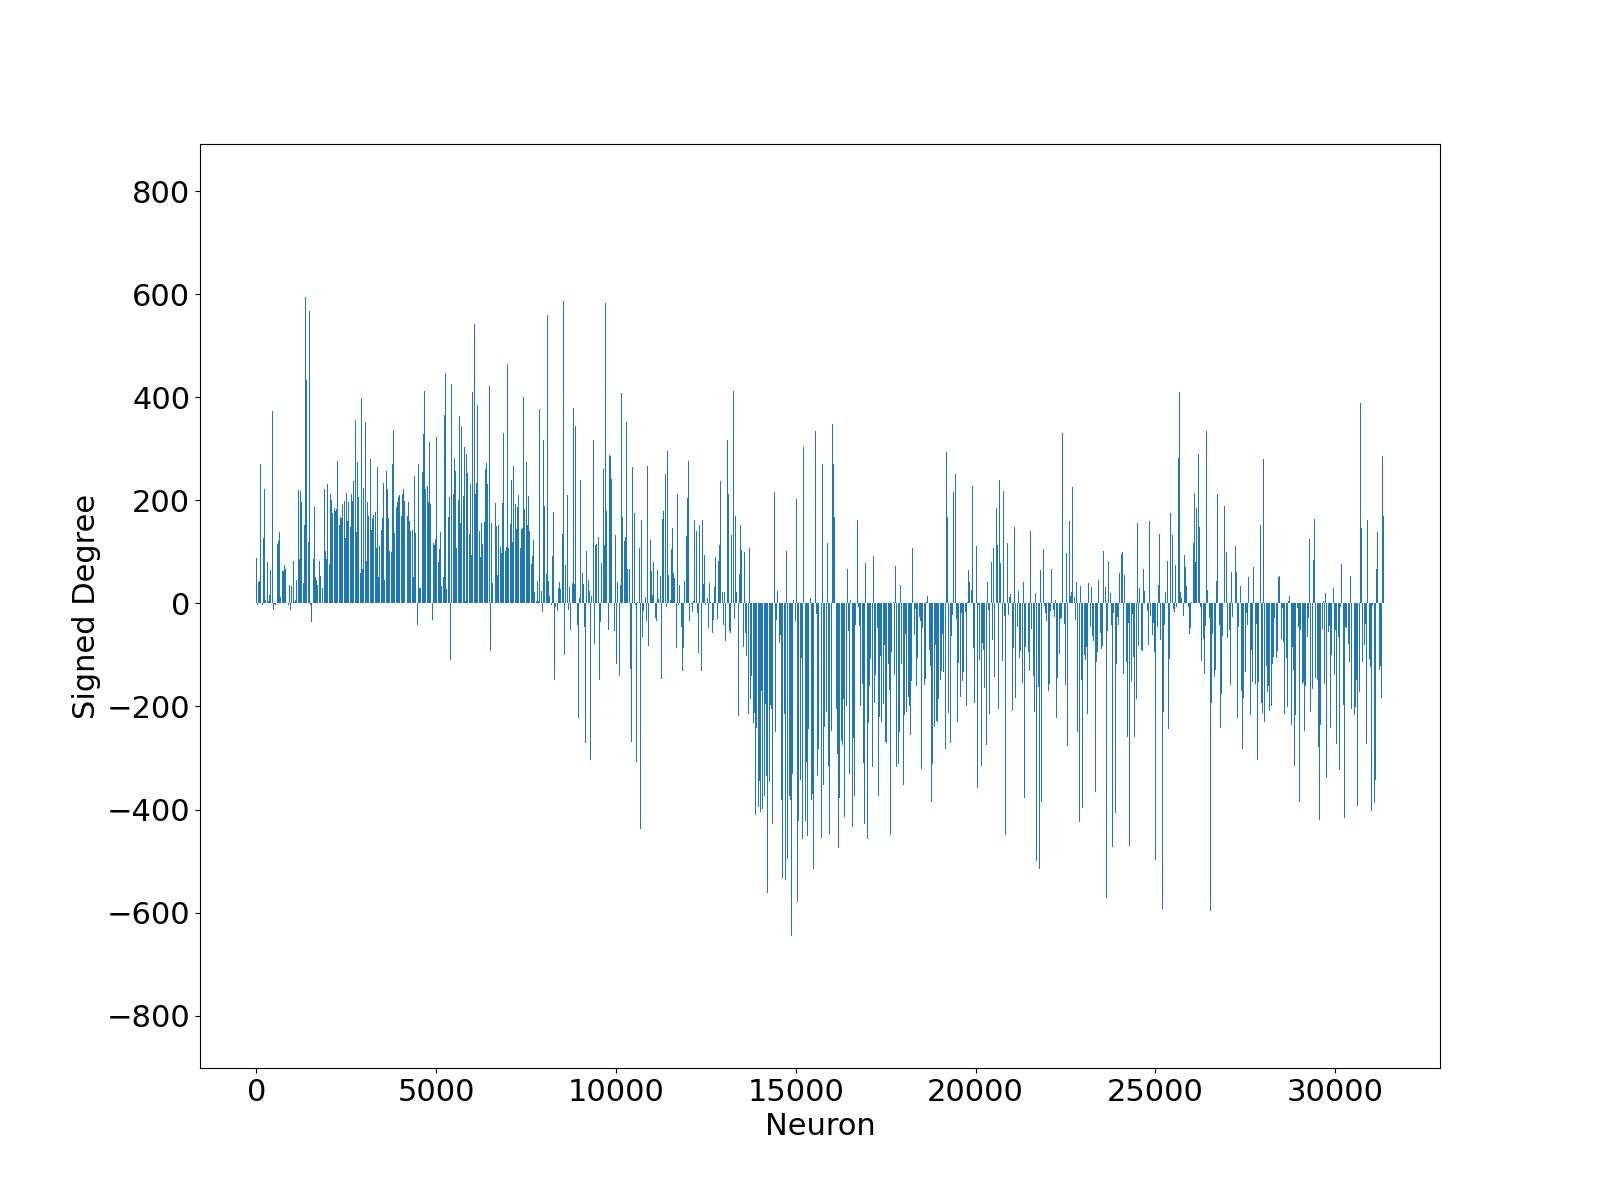
\includegraphics[width=7cm]{GBC/BGC_sd.png} }}%
    \qquad
    \subfloat[\centering Cumulative sum of the Signed Degree of the neurons in a realisation of the random graph $\mathcal{G}_{BGC}$]{{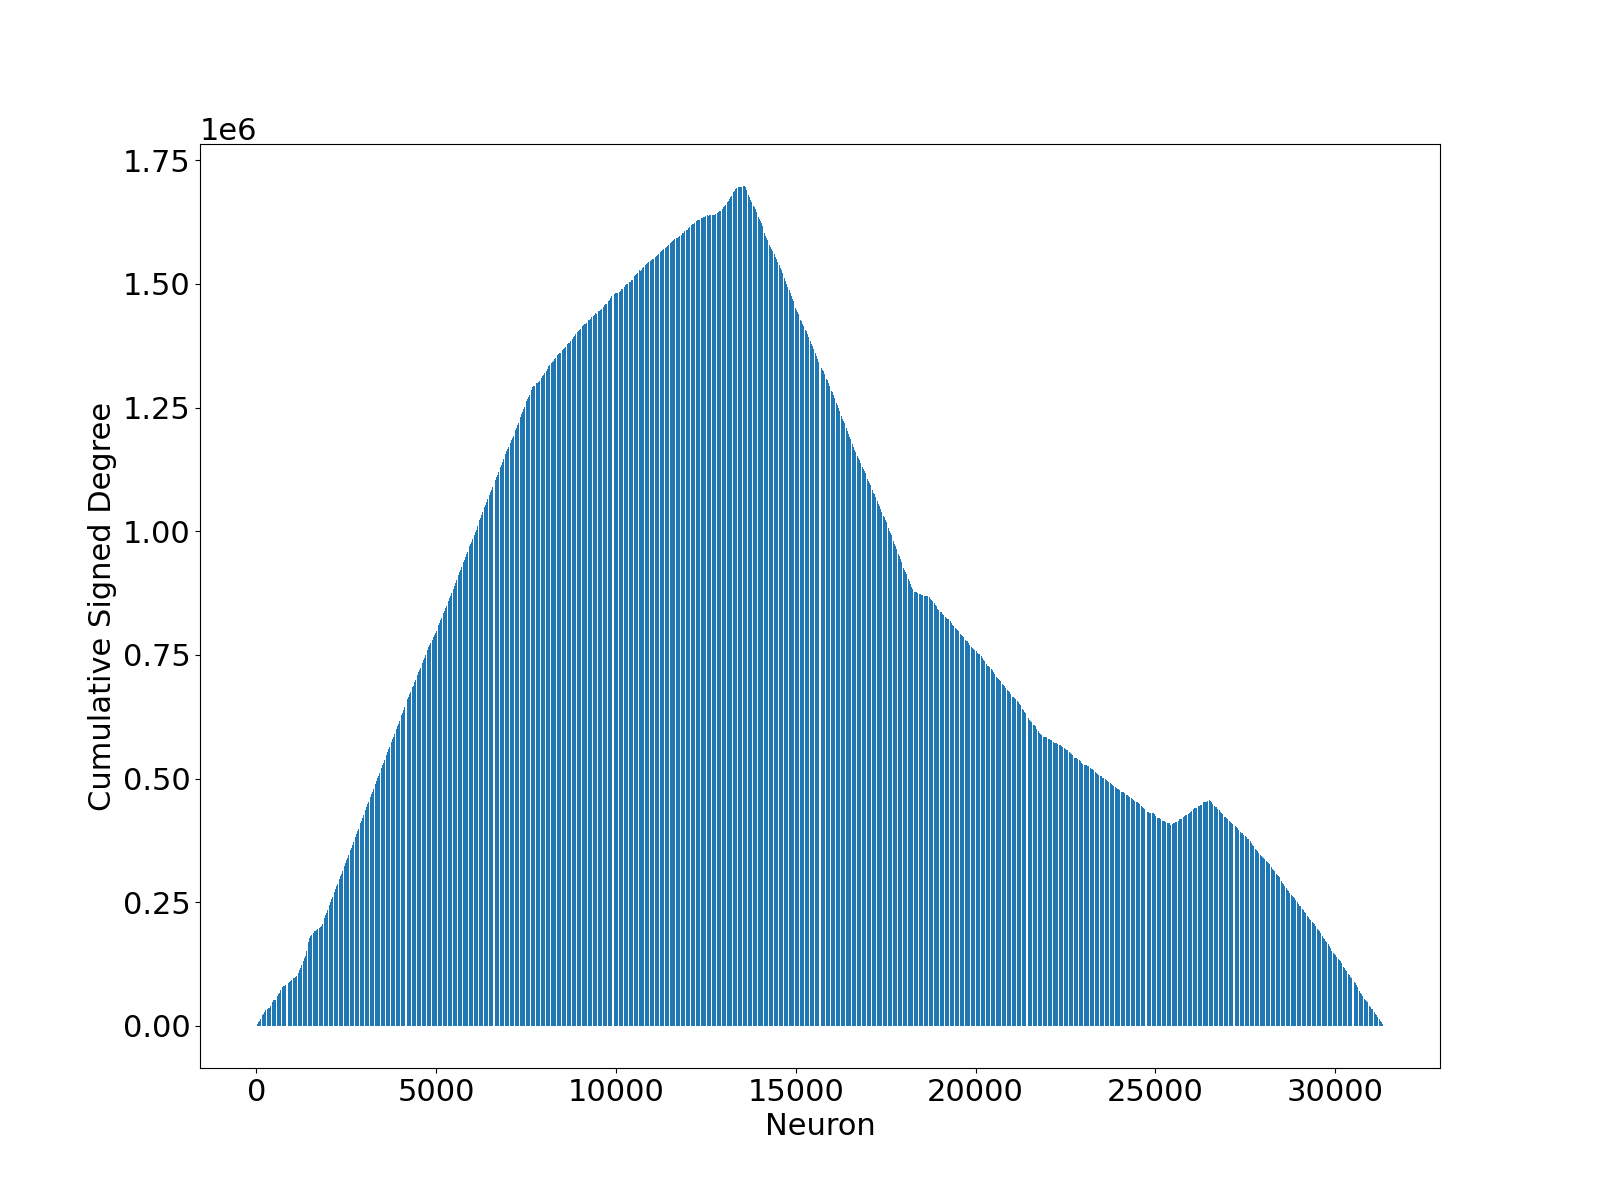
\includegraphics[width=7cm]{GBC/cumsum_degree_BGC.png} }}%
    \caption{Neuron statistics for the random graph $\mathcal{G}_{BGC}$}%
    \label{fig:example}%
\end{figure}



\newpage
\subsection{General Biological Model}
\subsubsection{The Model}
The General Biological model is the model that is proposed in the Frontiers article \cite{Reimann_2017}. 

\begin{figure}[H]
\begin{center}
\captionsetup{justification=centering}
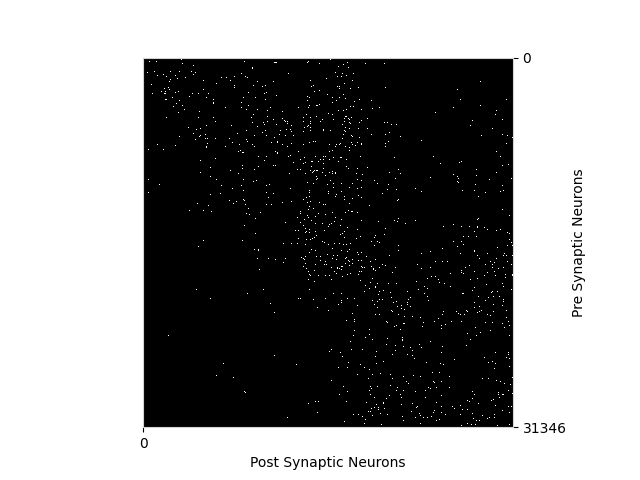
\includegraphics[width=12cm]{GB/matrix_general_biol.png}
\caption{Adjacency Matrix M representing a realisation of the random graph $\mathcal{G}_{GB}$}
\end{center}
\end{figure}

This model subdivides the MC into 3025 sub-matrices which represent each morphological neuron type from pre-synaptic to post-synaptic neurons. That is, we have 55 different morphological neuron types. Now, within these sub-matrices, we compute the distances between all pairwise neurons. These distances get binned, as mentioned in Section 4.1.3, into bin sizes of 75$\mu$m. Now, within these bins, we then shuffle the connections, so that a distance is preserved. We can see this diagrammatically in Figure 35. When the shuffling is completed, the sub-matrices are reassembled to form a complete matrix which now represents a realisation of the random graph $\mathcal{G}_{GB}$ given by the General Biological model. 

\begin{figure}[H]%
    \centering
    \captionsetup{justification=centering}
    \subfloat[\centering Connections in each morphological block]{{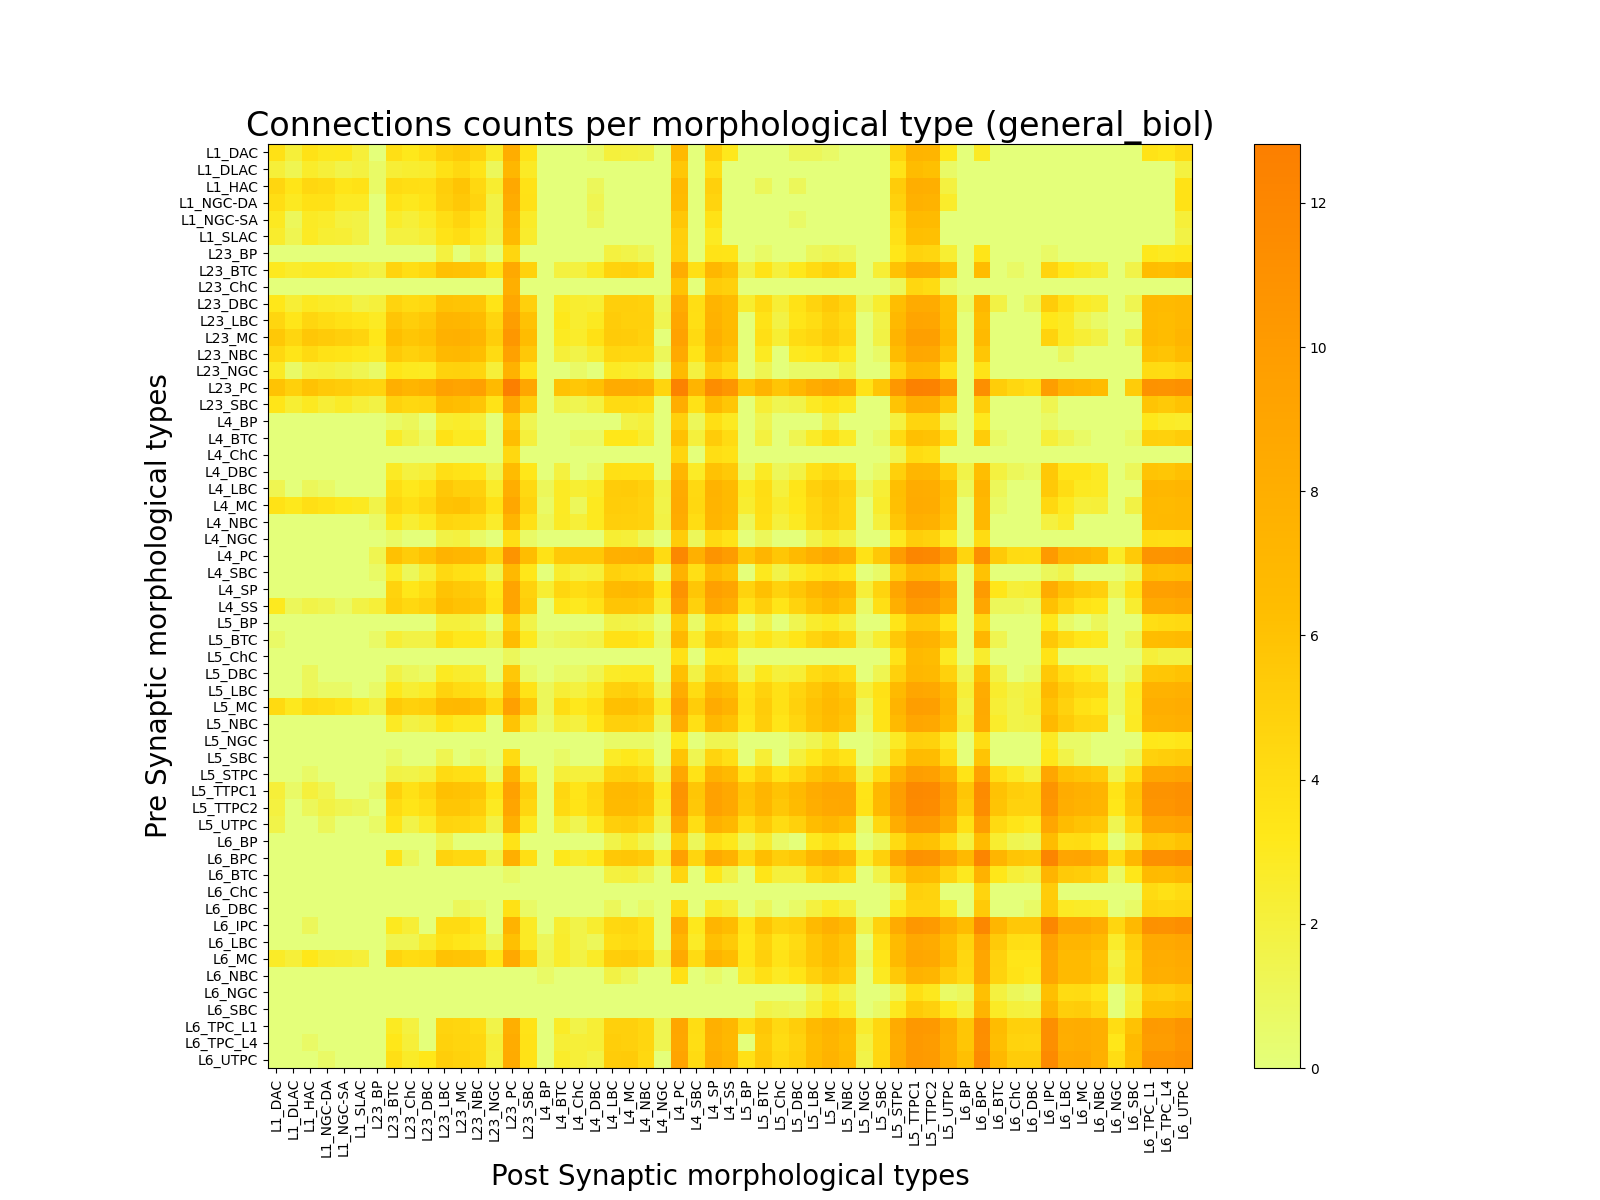
\includegraphics[width=7cm]{GB/heat_map_morph_layer_general_biol.png} }}%
    \qquad
    \subfloat[\centering A closer look at the morphological block L1\_DAC ]{{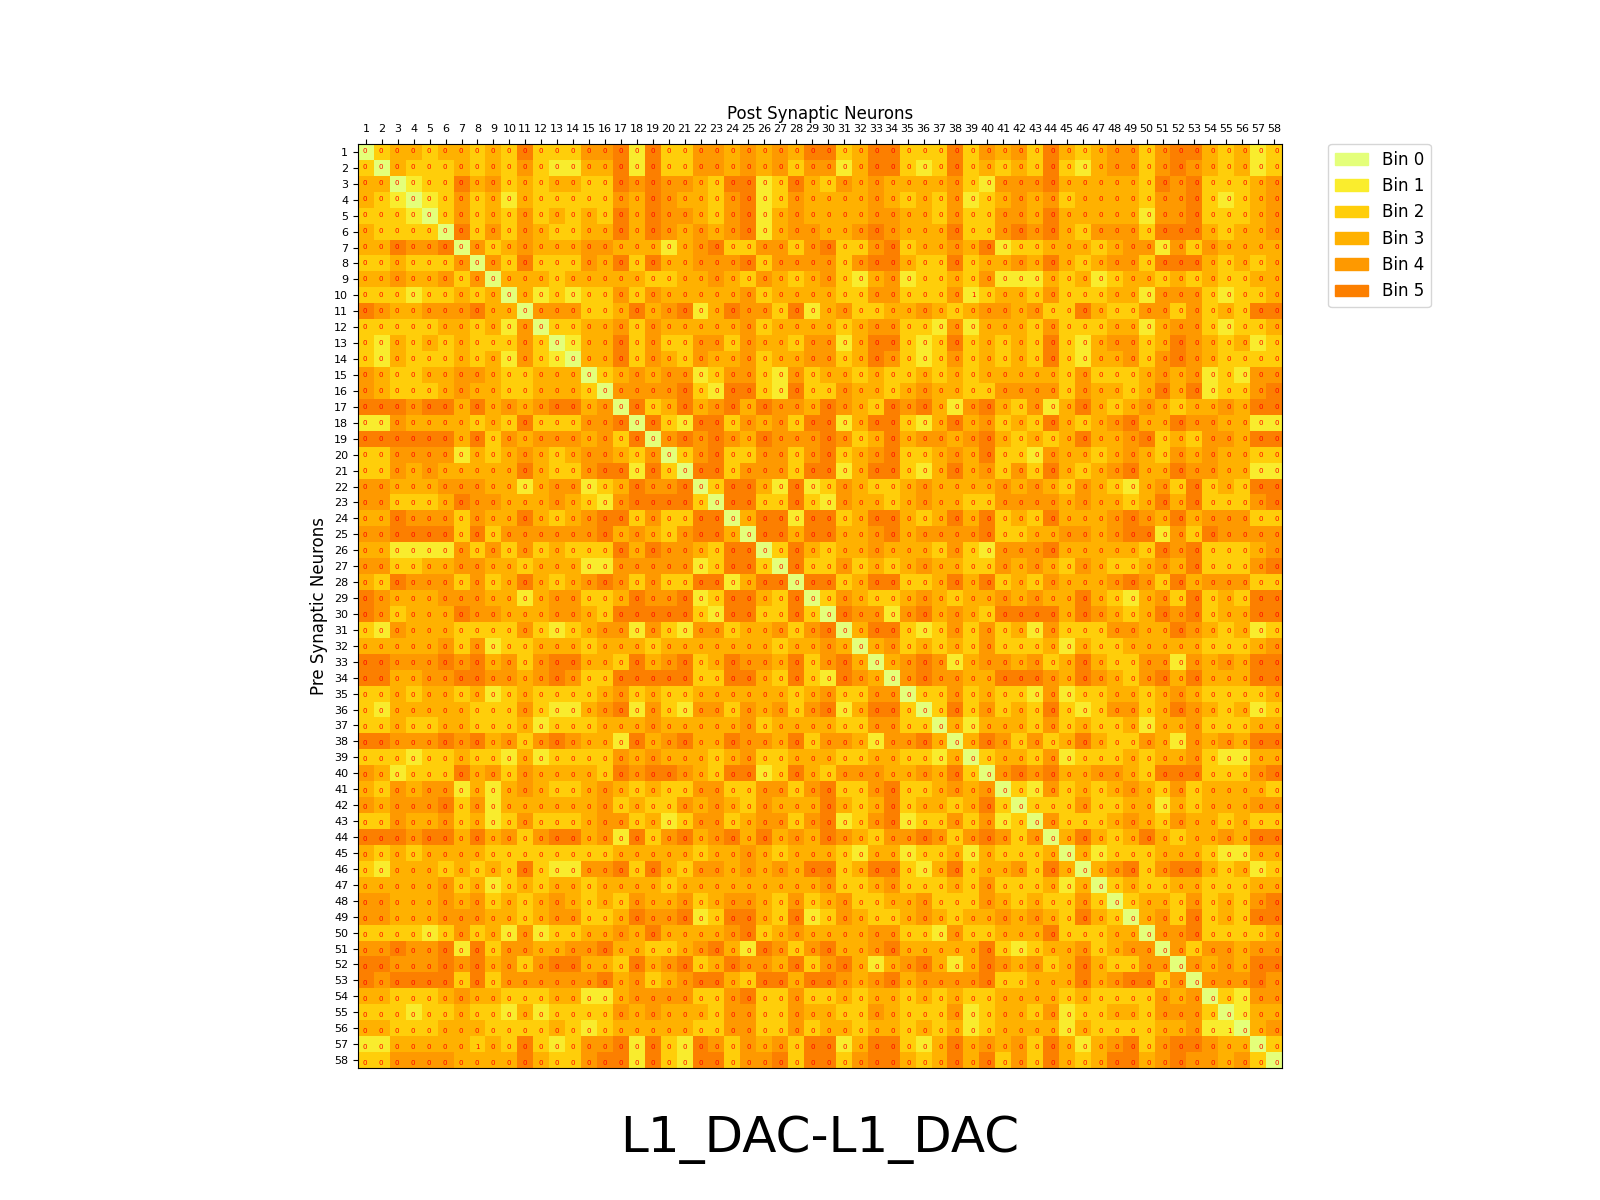
\includegraphics[width=7cm]{GB/L1_DAC.png} }}%
    \caption{Connectivity of GB Model}%
    \label{fig:example}%
\end{figure}

\begin{figure}[H]%
    \centering
    \captionsetup{justification=centering}
    \subfloat[\centering Sample of connected graph before shuffling]{{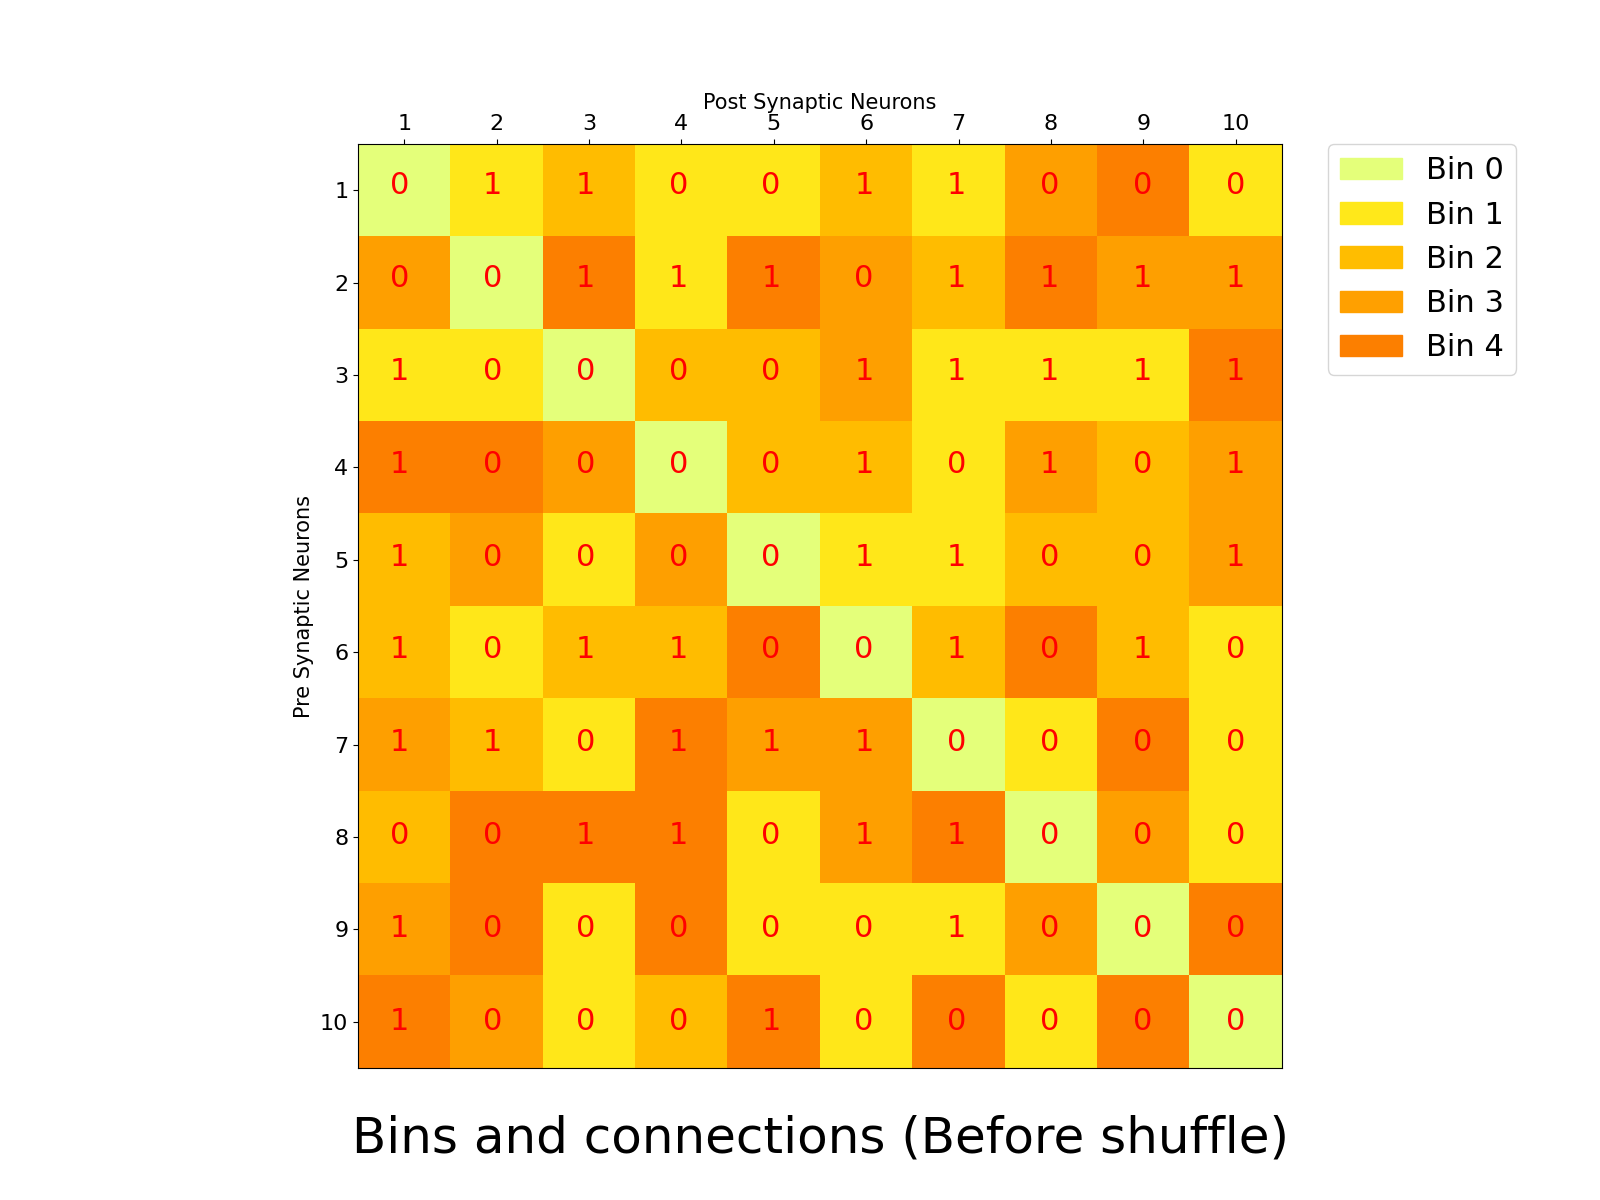
\includegraphics[width=7cm]{GB/before.png} }}%
    \qquad
    \subfloat[\centering The same sample after shuffling ]{{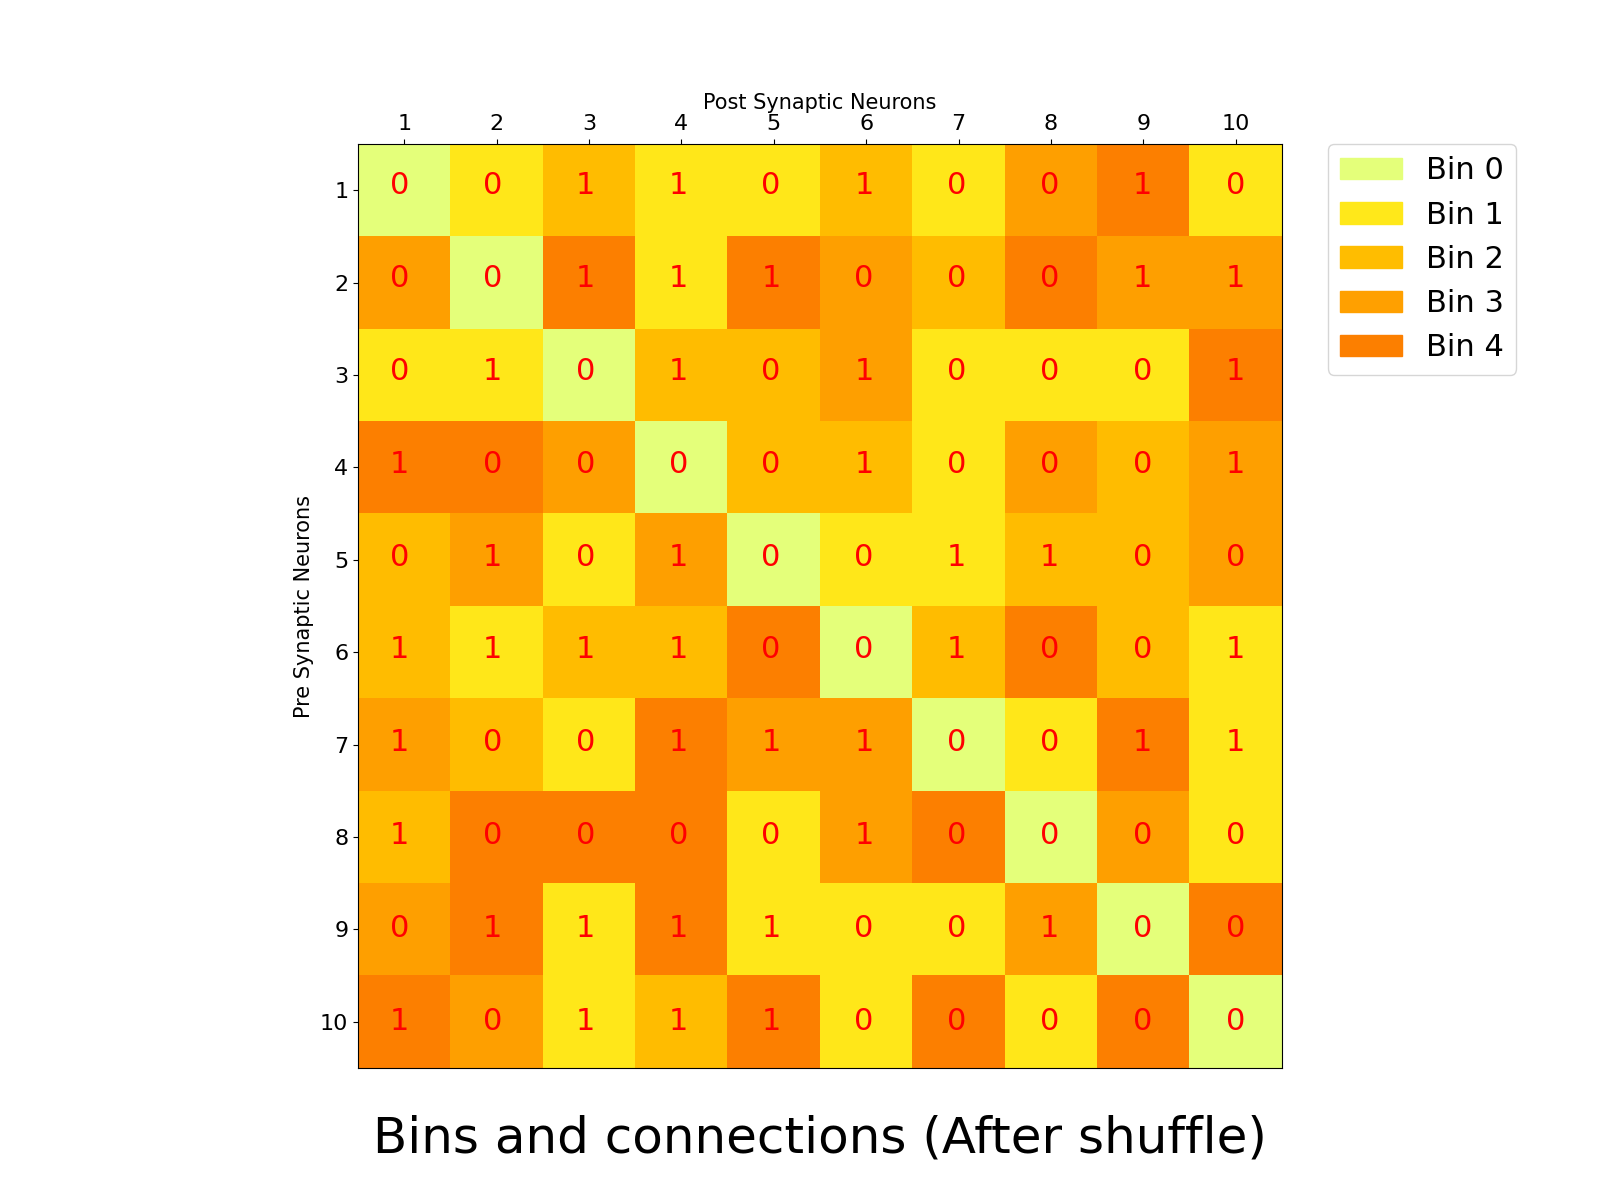
\includegraphics[width=7cm]{GB/after.png} }}%
    \caption{An example of a block before shuffling connections and after}%
    \label{fig:example}%
\end{figure}
Figure 34(a) represents the number of connections in each block. The blocks are split into morphological type. As we can see by the bar on the right hand side, darker shades show a block that is highly populated with connections and a lighter block representing a less populated block of connections. 
Figure 34(b) gives a representation of an individual morphological block, in this case L1 DAC, Layer 1 - Descending Axonal Collaterals, where we see pairwise neuron distances computed and binned according to a bin size of 75$\mu$m. The leading diagonal is the brightest shade of yellow and represents the smallest bin, that is a distance of 0$\mu$m and therefore are discounted, since they represent self-loops which do not exist. This leaves the remaining shades to be shuffled in each respective group. 
Figure 35(a) and 35(b) represent a sample shuffling of connections, whereby the connections and non-connections are shuffled within their respective bins as defined by the shades.
\subsubsection{Block Layouts}
Now, by restricting the connection shuffling to morphological neuron type blocks, which are subsets of the layer by layer blocks, we are able to maintain a Block-wise Edge density that is consistent with the Bio-M MC. Therefore, giving us a TV distance for Block-wise Edge Densities of 0. 

\begin{figure}[H]%
    \centering
    \captionsetup{justification=centering}
    \subfloat[\centering Block-wise Edge Densities]{{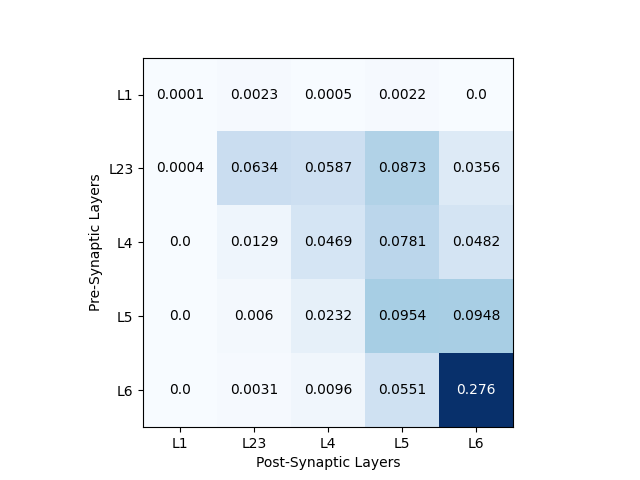
\includegraphics[width=7cm]{GB/heat_map_layer_gb_test.png} }}%
    \qquad
    \subfloat[\centering  Block-wise Edge Counts ]{{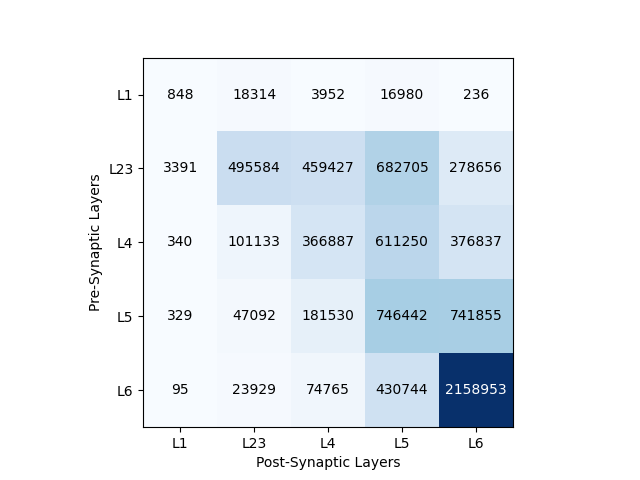
\includegraphics[width=7cm]{GB/heat_map_layer_general_biol.png} }}%
    \caption{Connectivity by block of the random graph $\mathcal{G}_{GB}$ given by the GB model}%
    \label{fig:example}%
\end{figure}

\subsubsection{Distance Distributions}
Figure 37 shows that with distance-dependence taken into account in the form of keeping bin sizes to a maximum size of $75\mu$m, we are able to maintain the exact same distribution as that of the Bio-M MC. In fact, we get a mean TV distance over 100 realisations, to be $\epsilon$. That is to say that the difference is statistically insignificant as a non-zero value occurred but once and was of the order $\epsilon < 1\times10^{-7}$. The details of the exact value is given in Section 6, Results.

\begin{figure}[H]
\begin{center}
\captionsetup{justification=centering}
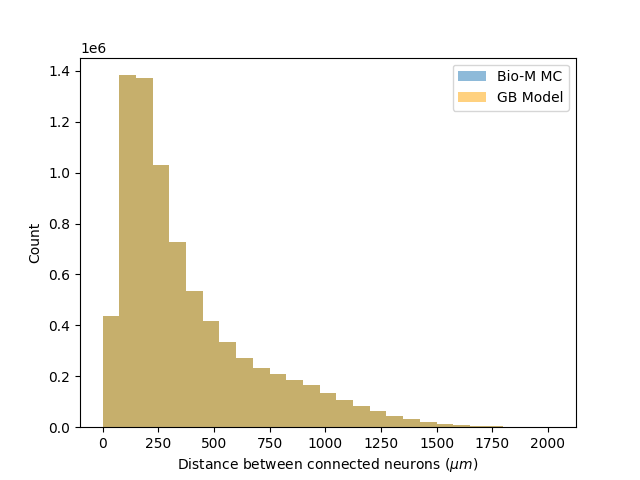
\includegraphics[width=12cm]{GB/general_biol_dist_distr.png}
\caption{Distance distribution of connected neurons for the random graph $\mathcal{G}_{GB}$}
\end{center}
\end{figure}

\subsubsection{Signed Degree of Neurons}
One curiosity that occurred when constructing the random graph for the General Biological model was the directionality upon computing the cumulative sum. This exhibited a different path to that of all other models, and hence why it is shown in Figure 38(b). The underlying reason for this will be that whilst the construction process restricted the MC into blocks of morphological type and shuffled connections here, the shuffling wasn't based on the pre-existing connections in the MC, but rather the distances between all neurons within each block and therefore creating entirely new sets of pre-synaptic and post-synaptic neurons. This therefore, does not preserve the in-degree and out-degree of each neuron.
\begin{figure}[H]%
    \centering
    \captionsetup{justification=centering}
    \subfloat[\centering Cumulative Signed Degree]{{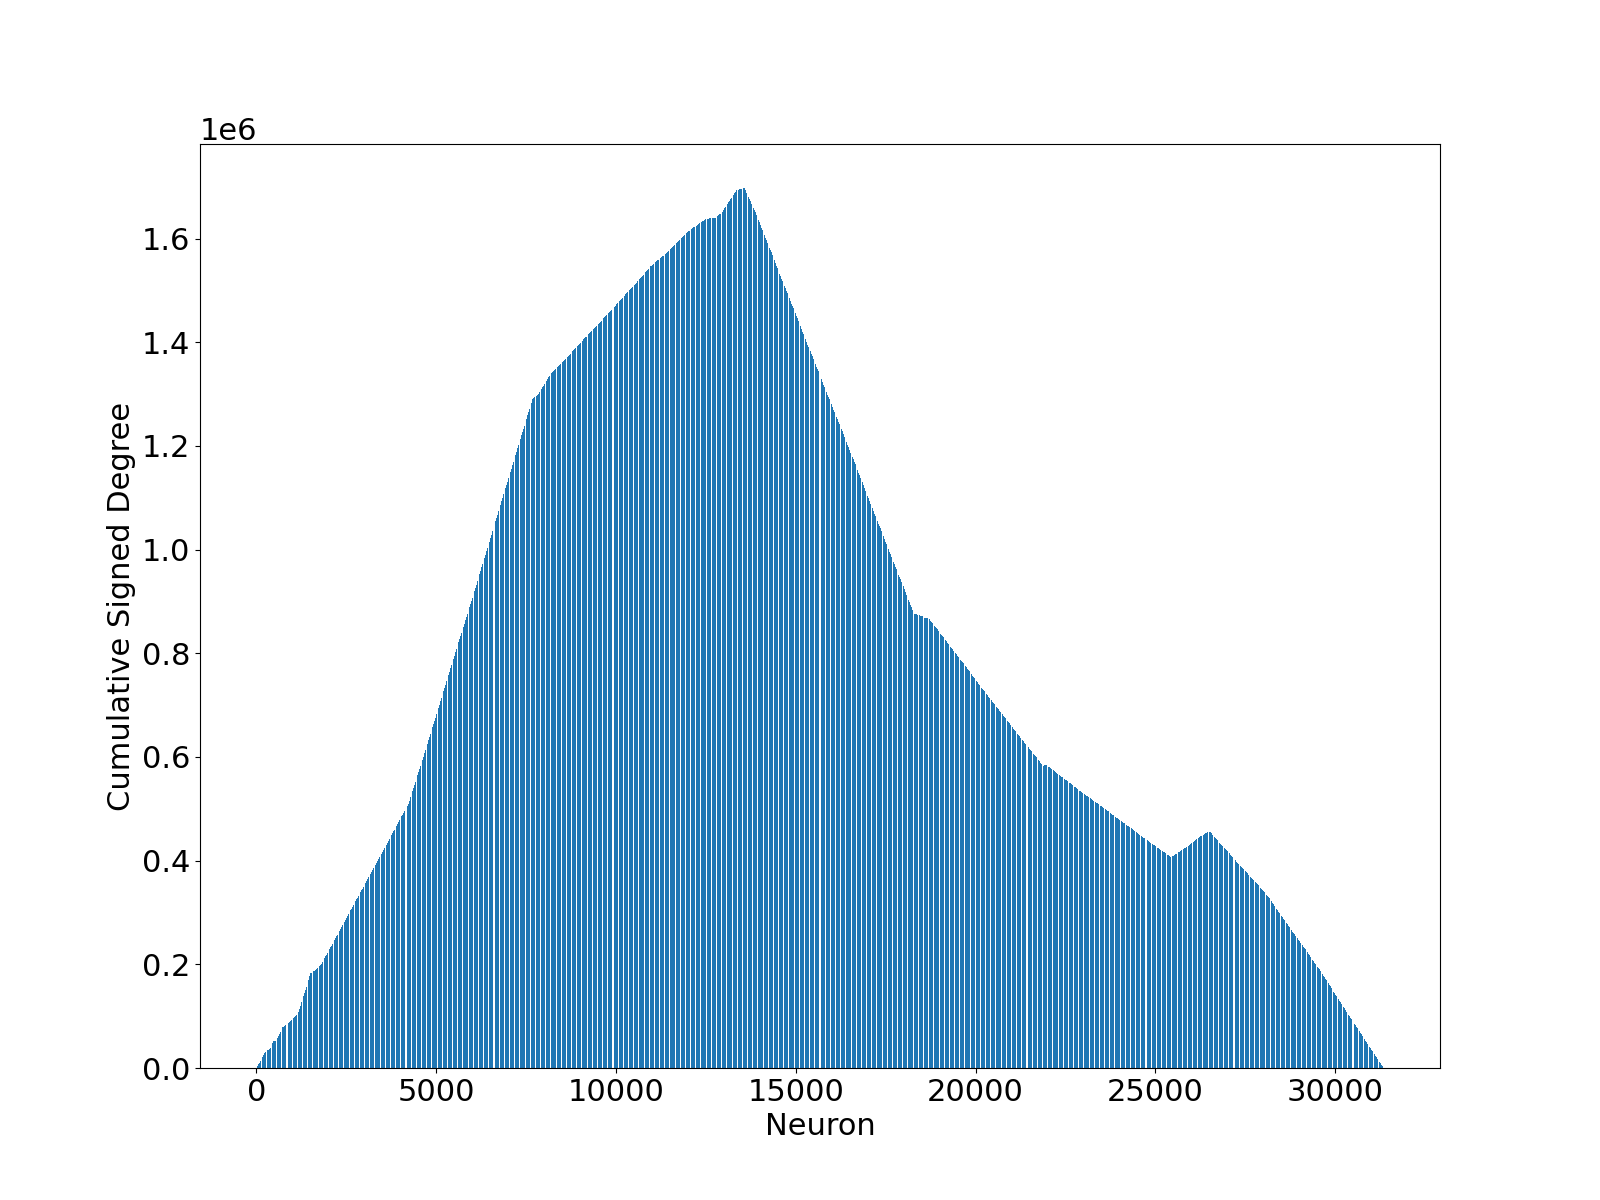
\includegraphics[width=7cm]{GB/cumsum_degree_general_biol.png} }}%
    \qquad
    \subfloat[\centering Directionality]{{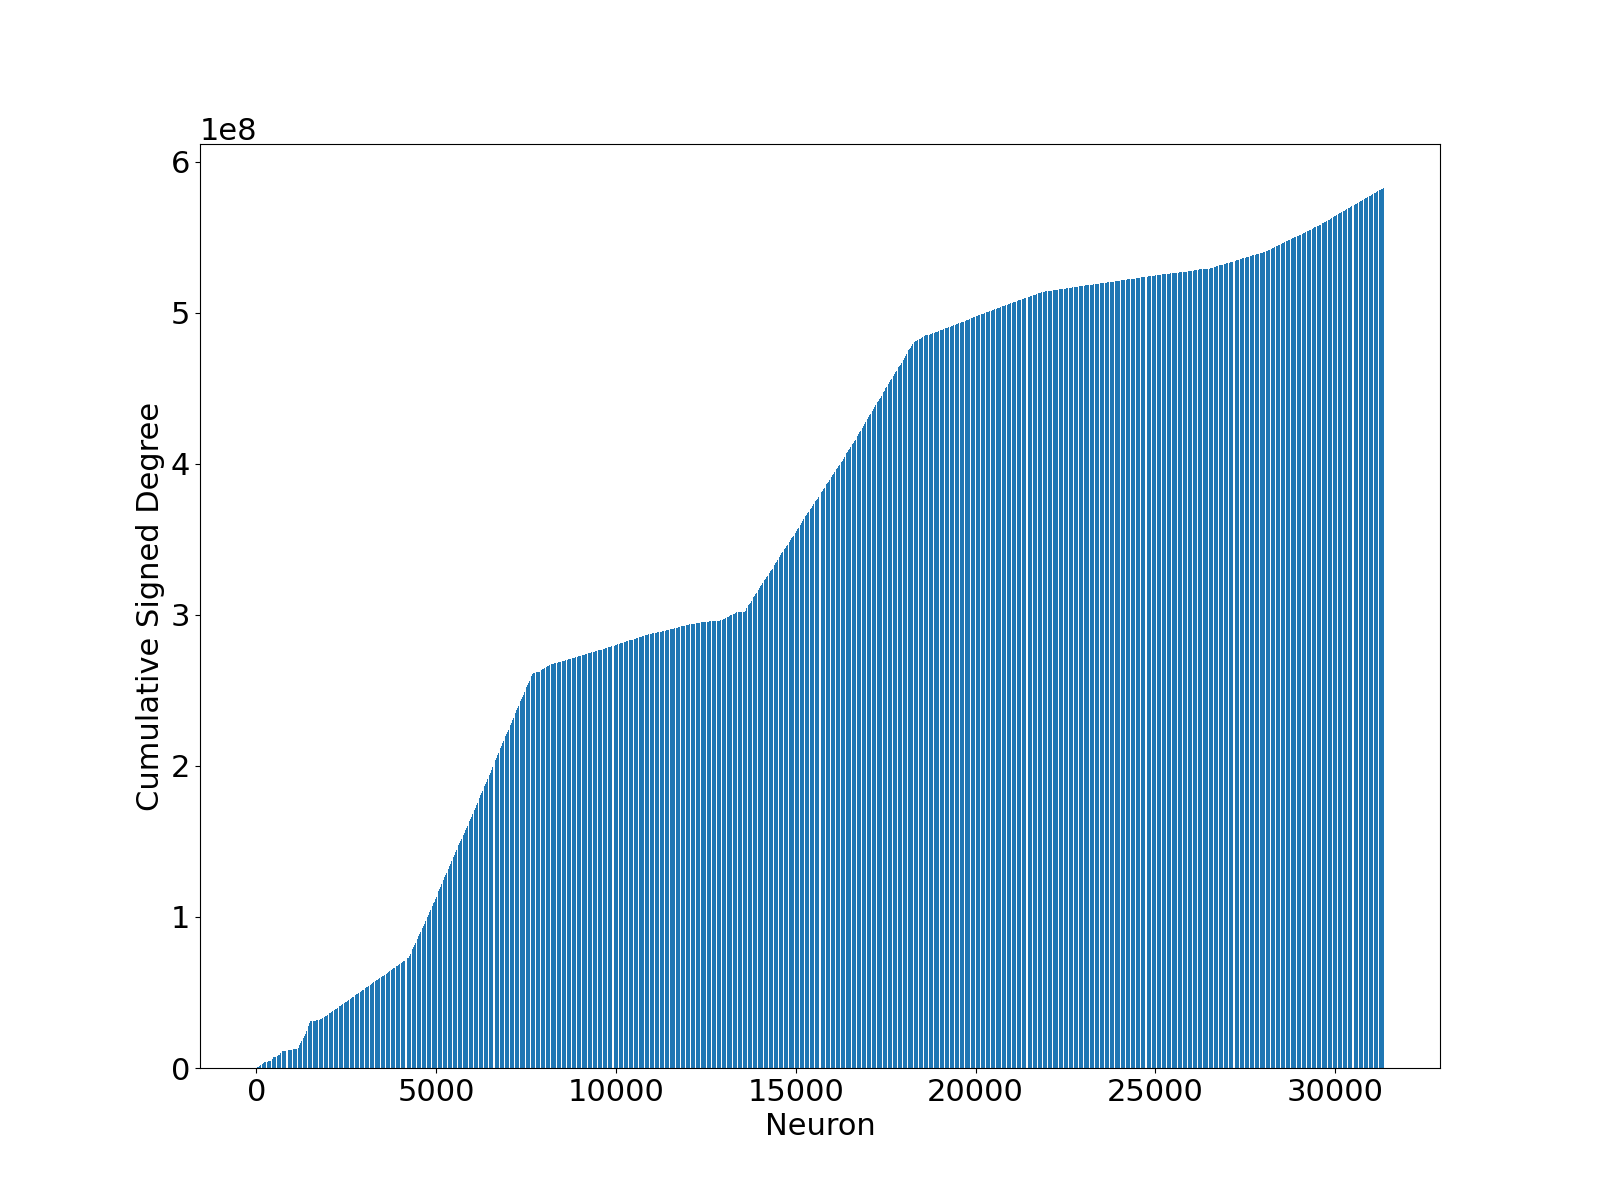
\includegraphics[width=7cm]{GB/overall_degree_general_biol_sd_2.png} }}%
    \caption{a sample of the cumulative signed degree and the directionality of the GB model}%
    \label{fig:example}%
\end{figure}